\documentclass[en]{../../../eplsummary}
\usepackage{framed}
\usepackage{placeins}
\usepackage{listings}
\usepackage{color}
\usepackage{fourier}
\usepackage[]{algorithmicx}

\definecolor{dkgreen}{rgb}{0,0.6,0}
\definecolor{gray}{rgb}{0.5,0.5,0.5}
\definecolor{mauve}{rgb}{0.58,0,0.82}

\DeclareMathOperator{\scp}{scp}
\DeclareMathOperator{\rel}{rel}
\DeclareMathOperator{\sol}{sol}

\lstset{frame=tb,
  language=Java,
  aboveskip=3mm,
  belowskip=3mm,
  showstringspaces=false,
  columns=flexible,
  basicstyle={\scriptsize\ttfamily},
  numbers=none,
  numberstyle=\tiny\color{gray},
  keywordstyle=\color{blue},
  commentstyle=\color{dkgreen},
  stringstyle=\color{mauve},
  breaklines=true,
  breakatwhitespace=true,
  tabsize=3
}

\graphicspath{{res/}}

\hypertitle{algo-INGI2266}{7}{INGI}{2266}
{Houtain Nicolas}
{de Vogelaere Cyril}
{Gusbin Quentin}
{Pierre Schaus}

\section{Dynamic programing}

\subsection{Definition}

\textbf{Dynamic programming} is a method by recurrence in order to solve complex problem.
\begin{itemize}
    \item breaking it down into a collection of simpler subproblems
    \item solving each of those subproblems just once, and storing their solutions in memory
    \item[$\rightarrow$] Next time the same subproblem occurs, instead of 
recomputing its solution, only looks up to the previously computed solution.
Thereby \textbf{saving computation time at the expense of storage space}.
\end{itemize}

\subsection{Solving the knapsack problem with DP}

\subsubsection{The knapsack problem}
\begin{itemize}
    \item A set of item $I$
    \item for each item $i \in I$ is associated a value $v_i$ and a weight $w_i$.

    \item[Goals] 
        \begin{tabular}{m{3cm}m{12cm}}
            $\sum_{i \in I} v_i x_i$: & Maximize the value of selected items\\
            $\sum_{i \in I} w_i x_i \le C$ & Under constraint that the total
            capacity cannot exceed a given maximal capacity $C$ \\ 
            $x_i \in \{0,1\}$ & And an item cannot be partially selected \\
        \end{tabular}
\end{itemize}

Note that Knapsack is an NP-Complete problem as it can be used
to find a solution to the subset-sum problem, which is NP-complete.

\paragraph{Subset-sum problem}

Given a set of natural number and a capacity K. 
Find a subset S such that :
$$\sum_{i \in S} c_i = K$$


\subsubsection{Solutions}
\begin{itemize}
    \item \textbf{DP for knapsack in 0(Cn)}.

        Refer to the optimal objective of the problem with capacity $k$ and
        items \{1,…,j\} $\in$ I as $O(k,j)$. We can easily notice that :

        \begin{itemize}
            \item $O(k,0) = 0 \text{\footnotemark}$
            \item $ O(k,j) = \begin{cases} 
                    max(O(k,j-1) , vj +O(k-wj,j-1))\text{\footnotemark} & if \quad w_j \leq k \\
                    O(k,j-1) & otherwise
                \end{cases}$
        \end{itemize}
        \footnotetext{As their are no elements to choose from}
        \footnotetext{Bellman's equations}


        \begin{lstlisting}[caption=Knapsack DP]
val items = Array((1,1),(6,2),(18,5),(22,6),(28,7)) // (value,weight)
val C = 11
def O(j: Int, k: Int): Int = {
    if (j < 0) 0
    else {
        val (vj,wj) = items(j)
        if (wj > k) O(j-1,k)
        else O(j-1,k).max(vj + O(j-1,k-wj))
    }
}
println(O(items.size-1,C))
        \end{lstlisting}

        \begin{center}
    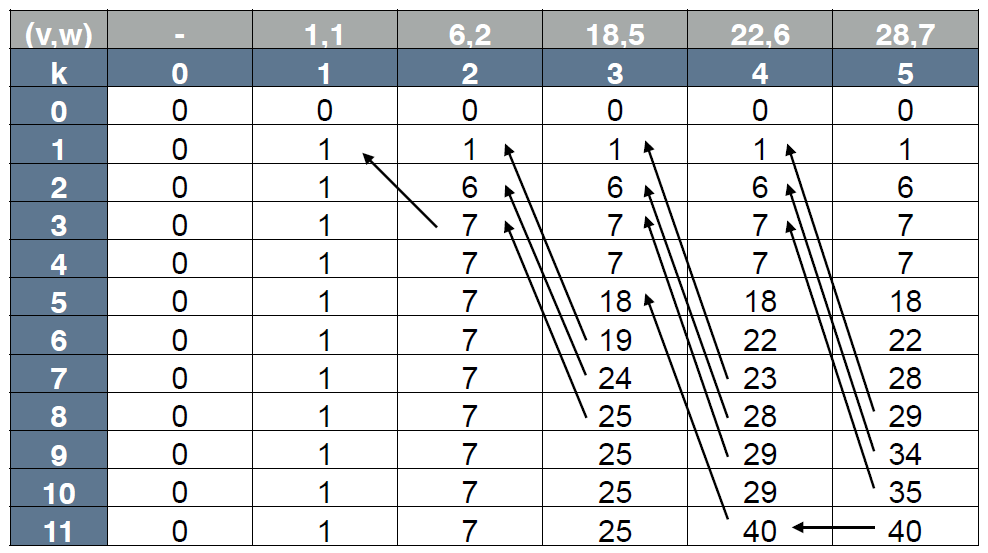
\includegraphics[width=7cm]{KnapsackDP.png}
        \end{center}

    \item \textbf{DP for knapsack in 0(Vn)}.

        Using a similar logic, it is also possible to define an algorithm which
        run in $\theta$(Vn) to compute knapsacks. Let $V = \sum_{i \in I} v_i$,
        we can redefine O(k,j) as O(w,j), the optimal weight using only items
        \{1,...,j\}. The equation will thus change as follow :

    \begin{itemize}
    \item $O(0,j) = O(w,0) = 0 \text{\footnotemark} $
    \item $ O(w,j) = \begin{cases}
                min(O(w,j-1), wi + O(w-v_j,j-1)) & if \quad v_j \leq p \\
                O(w,j-1) & otherwise
            \end{cases}$
        \end{itemize}
        \footnotetext{As $w_i > 0$ for all $i \in I$ and as we cannot have w > 0 with 
        an empty set.}
        \begin{center}
            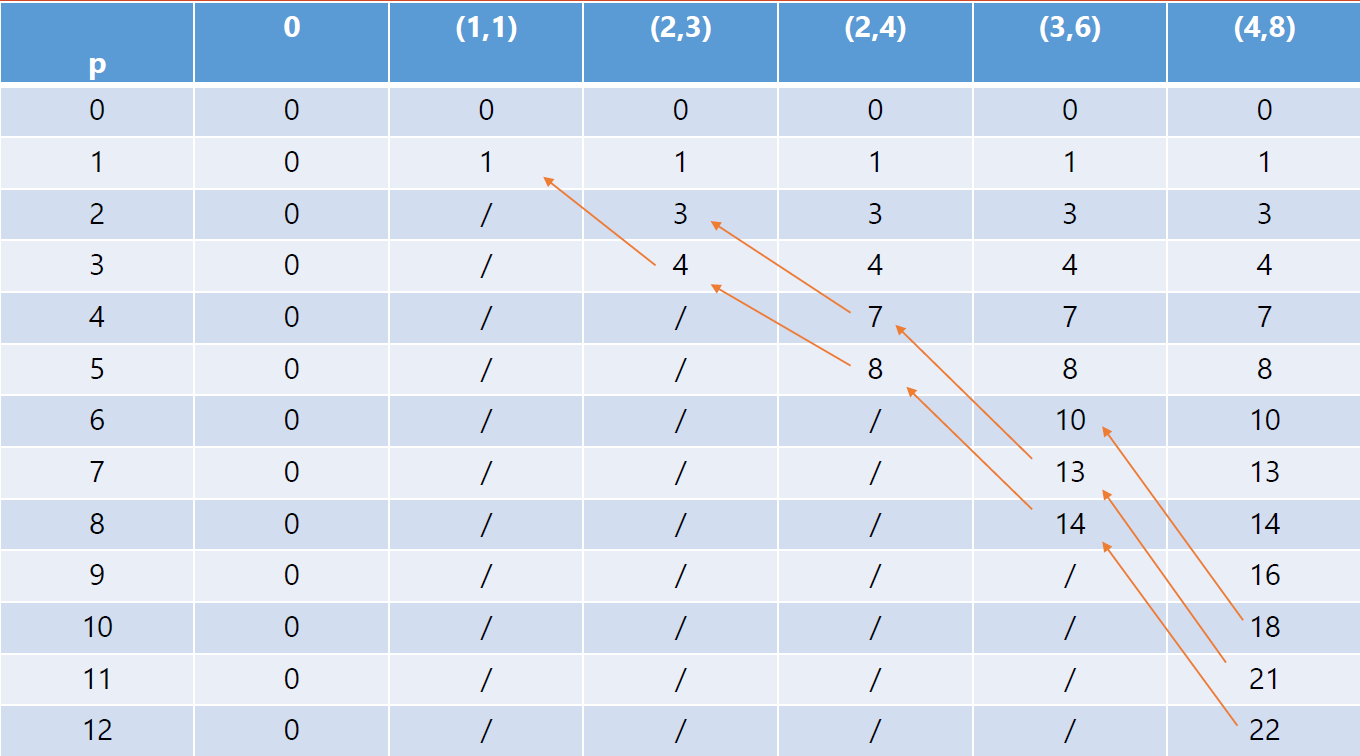
\includegraphics[width=7cm]{KnapsackDPAlgo2.png}
        \end{center}
\end{itemize}

\subsubsection{Cache usage}
\begin{tabular}{m{9cm}m{6cm}}
As explain, a cache is use in order to store computed value and avoid to recompute
it. In \textcolor{red}{red} we have the cells actually computed.
&
    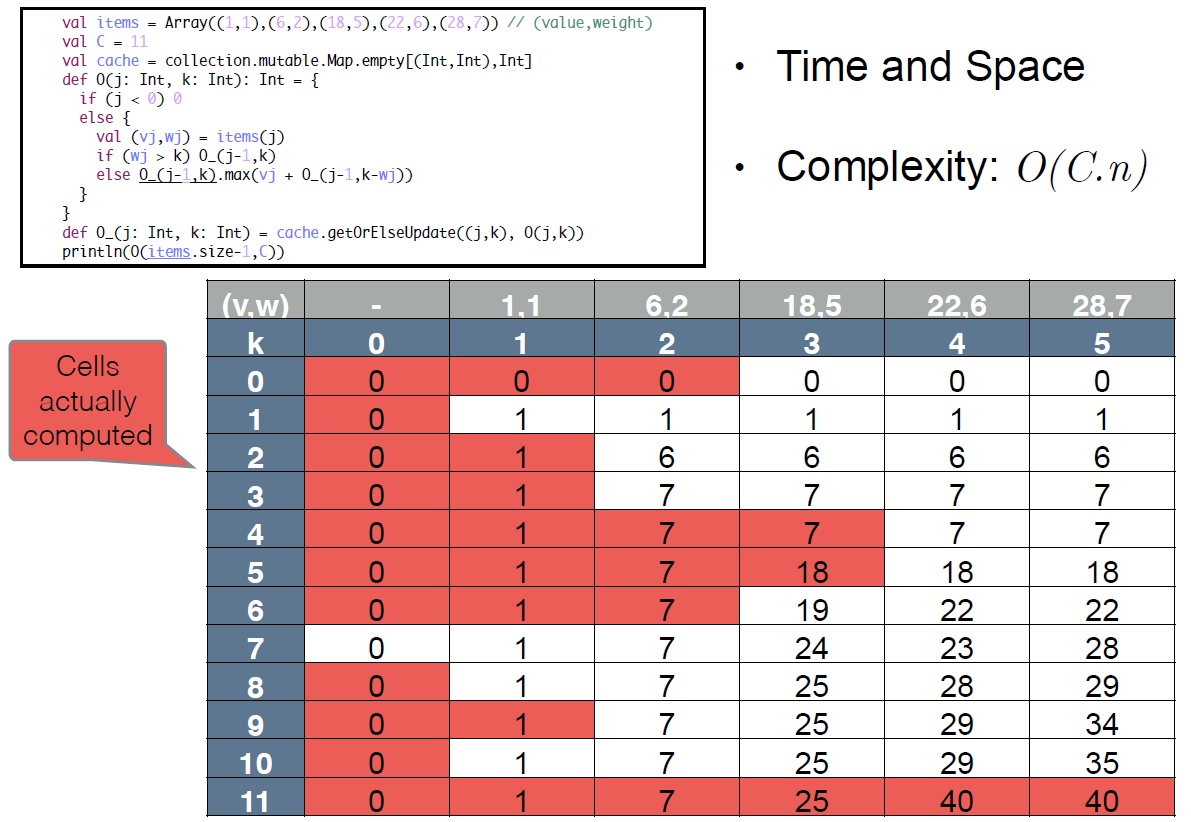
\includegraphics[width=6cm]{KnapsackDPAlgo1.png}
\end{tabular}


\subsubsection{Pseudo-polynomial}

DP is \textsc{pseudo-polynomial}, since it is exponential in the 
\textit{length of input} ($log(C)$) which is the number of bits required to
encode the input ($C$). The complexity is thus exponential relatively to the
input size. This algorithm is \textbf{weakly NP-Complete} or
\textbf{pseudo-polynomial}\footnote{a numeric algorithm runs in
pseudo-polynomial time if its running time is polynomial in the numeric value
of the input, but is exponential in the length of the input – the number of
bits required to represent it.} as it is roughly polynomial for small values of
C while computing larger value is much more expensive\footnote{Not all
    NP-Complete algorithm are pseudo polynomial ! Like the traveling salesman
problem (TSP), for example.}.


\subsection{Other examples of DP algorithms}

Before reading this section, please remember that all algorithm that can be
implemented via dynamic programming are not ipso-facto pseudo polynomial ! Any
algorithm can be expressed with dynamic programming as long as it can be separated in
sub problems.

\subsubsection{Edit distance}


TODO

\subsubsection{TSP}
 
TODO



\subsection{Exam}
I give you a problem (for instance the TSP, Knapsack)
\begin{itemize}
    \item  Design a greedy algorithm
    \item  Design a Dynamic Programming formulation
    \item  Design a relaxation and upper/lower bound
        procedure and embed it in a Branch and Bound
    \item  Justify advantages and disadvantages of each
    \item  Apply the three techniques to a small instance
        manually
\end{itemize}


\section{Branch and bound}

\subsection{Definition}

A \textbf{branch-and-bound} algorithm consists of a systematic enumeration of candidate solutions by means of state space search: the set of candidate solutions is thought of as forming a rooted tree with the full set at the root. The algorithm explores branches of this tree, which represent subsets of the solution set. Before enumerating the candidate solutions of a branch, the branch is checked against upper and lower estimated bounds on the optimal solution, and is discarded if it cannot produce a better solution than the best one found so far by the algorithm.

\subsection{Solving the knapsack problem with B\&B}

Given the following knapsack problem :

\begin{figure}[!ht]
    \centering
    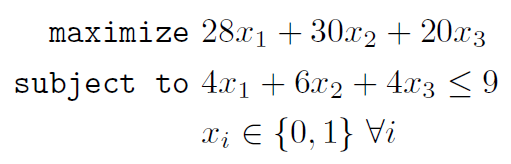
\includegraphics[width=0.4\linewidth]{KnapsackBBProblem.png}
    \label{fig:Knapsack_example}
\end{figure}
\FloatBarrier

We can choose to relax either of the constraint during the branch and bound procedure 
as to obtain a solution. The goal being to reduce the search space as much as possible
by calculating an upper bound as precise as possible.
Let us thus compare both options in the following sections.

\subsubsection{Capacity relaxation}

The first constraint that we can relax is the capacity constraint. The B\&B
calculation becomes fairly simple to implement as we only cut at tree branch when 
we have surpassed the capacity. The search space is thus reduced as such :

\begin{figure}[!ht]
    \centering
    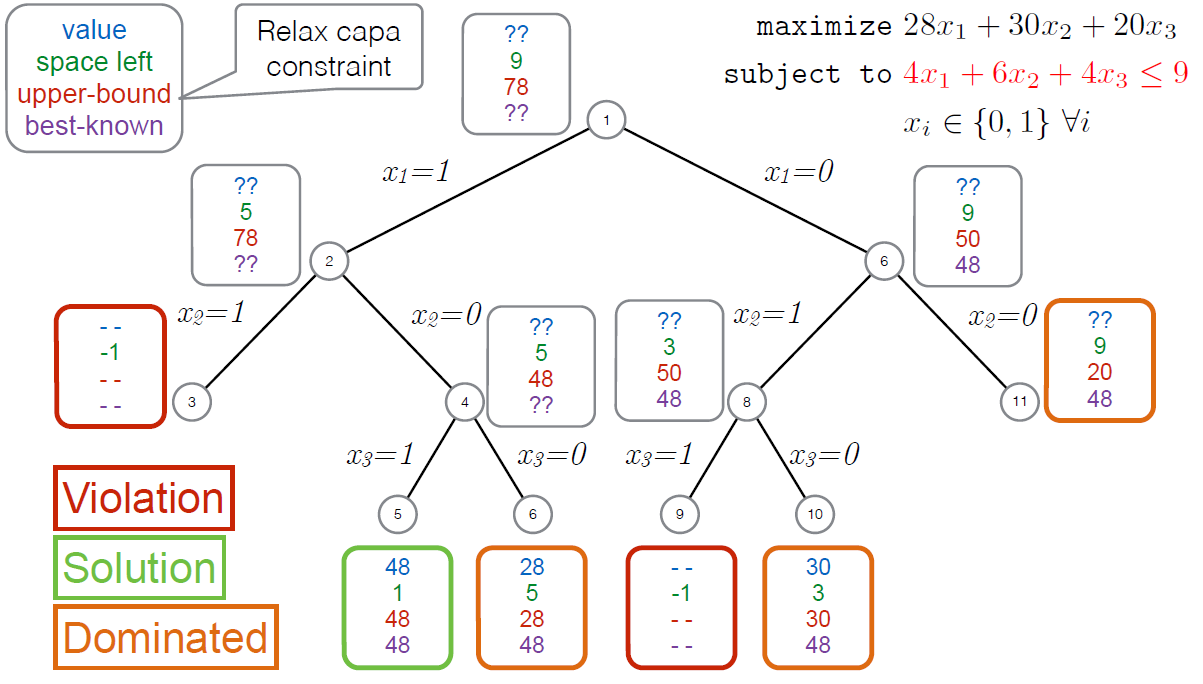
\includegraphics[width=\linewidth]{KnapsackBBCapaRelaxation.png}
    \label{fig:Knapsack_example}
\end{figure}
\FloatBarrier

Which, as you can see, is far from optimal as our upper bound are not close enough to their
real value.

\subsubsection{Linear relaxation}

This second relaxation is slightly harder to implement but yields better result, as 
the upper bound approximation is far better. Given a set sorted by ratio $v_i/w_i$,
the upper bound calculation procedure become as search for the first critical item j.
\newline

The first critical item j being the first item which cannot be fully added in our selection
due to capacity constraint. 

\begin{figure}[!ht]
    \centering
    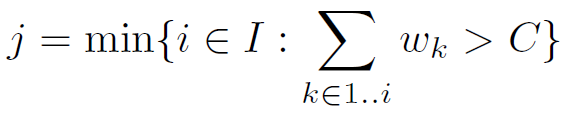
\includegraphics[width=0.4\linewidth]{KnapsackBBCriticalItem.png}
    \label{fig:Knapsack_example}
\end{figure}
\FloatBarrier

The upper bound can then be calculated as the sum of all item i < j plus as much of j
as we can squeeze in while respecting the capacity constraint.

\begin{figure}[!ht]
    \centering
    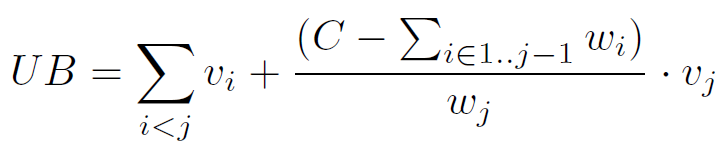
\includegraphics[width=0.5\linewidth]{KnapsackBBLinearRelaxationUB.png}
    \label{fig:Knapsack_example}
\end{figure}
\FloatBarrier

The search space is thus reduced as such :

\begin{figure}[!ht]
    \centering
    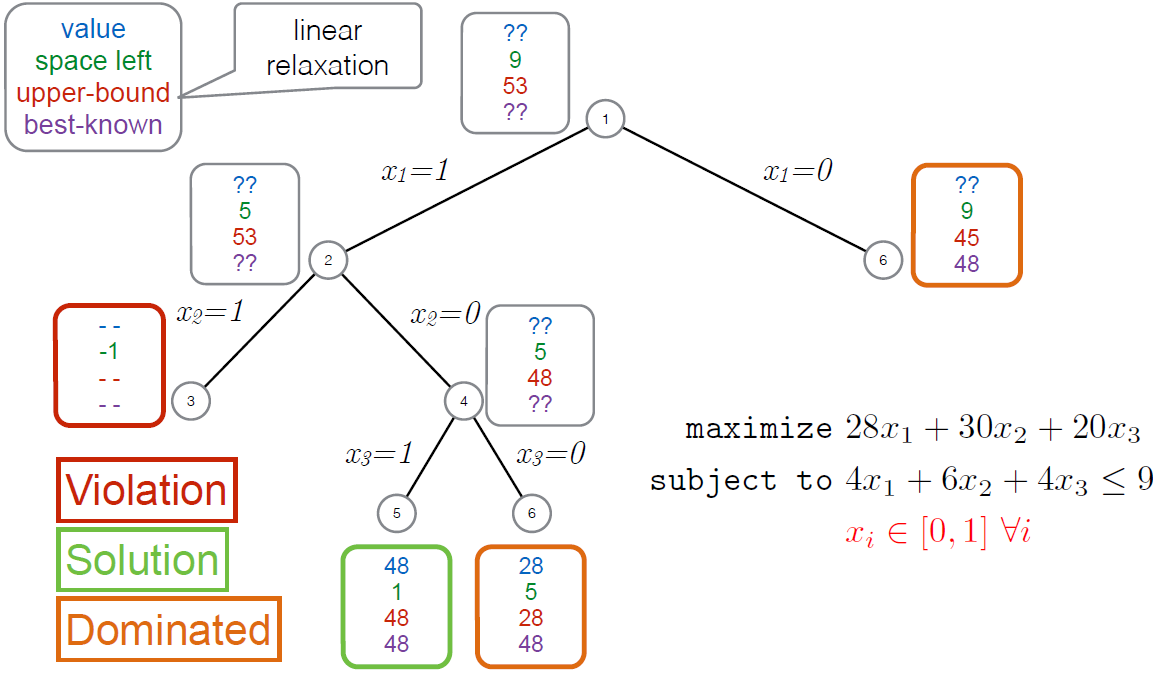
\includegraphics[width=\linewidth]{KnapsackBBLinearRelaxation.png}
    \label{fig:Knapsack_example}
\end{figure}
\FloatBarrier

As you can see, improving the precision of the upper-bound yields far better result. Take care however not to over/under estimate it (depending if you are on a maximisation or minimisation process) as it might prevent you to find the optimal solution.





\section{Linear programming}
\subsection{Definition}

Linear programming consist of a maximisation of a linear fonction subject to linear constraints.

\subsubsection{Example}

\begin{tabular}{m{8cm}m{5cm}}
    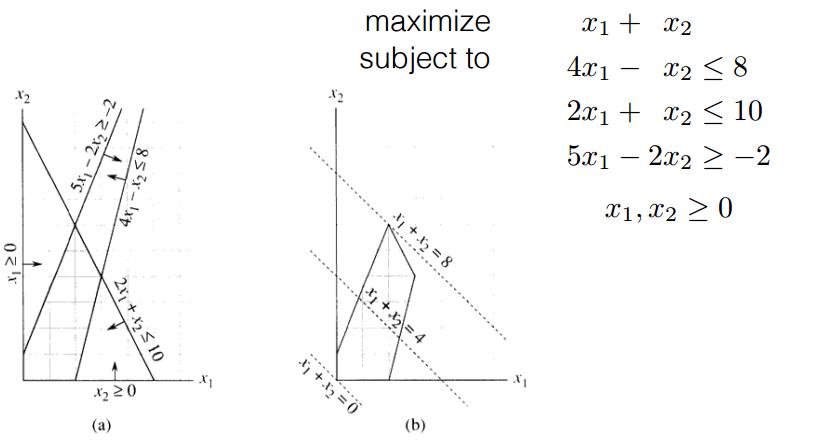
\includegraphics[width=7cm]{example1.png}
    &
    \begin{eqnarray*}
        \textrm{maximize } & x_1 + x_2 \\
        \textrm{subject to } & 4x_1 - x_2 & \leq 8 \\
                             & 2x_1 + x_2 & \leq 10 \\
                             & 5x_1 - 2x_2 & \geq -2\\
                            & x_1, x_2 \geq 0
        \end{eqnarray*}
\end{tabular}

\subsection{Polytope}

The solution space is a \textbf{polytope}. In a polytope, every point is a convex
combination of its vertices:
$$(\alpha x + (1 - \alpha)y) \in S \, \quad  with \quad \, \alpha \in
[0,1]$$

\begin{tabular}{m{8cm}m{4cm}}
    \begin{eqnarray*}
        \textrm{maximize } & c_1x_1 + ... + c_nx_n \\
        \textrm{subject to } & a_{11}x_1 + ... + a_{1n}x_n \leq b_1 \\
                             & ... \\
                             & a_{m1}x_1 + ... + a_{mn}x_n \leq b_m \\
        \end{eqnarray*}
        &
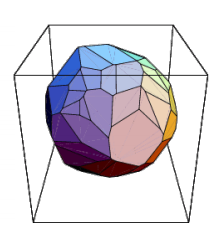
\includegraphics[width=3cm]{polytope.png}
\end{tabular}


\subsubsection{Theorem}
At least one of the points where the objective value is maximal is a vertex of the polytope.
\paragraph{Proof} : 
\begin{itemize}
    \item The maximum $x^{*}$ as a combination of the vertices of the
        polytope $v_{1},...,v_{t}$)
        $$x^{*} = \lambda_{1} v_{1} + ... + \lambda_{t} v_{t}$$

    \item Objective value at optimality can be expressed as a scalar
        product with $c$ a vector
        and the objective value at optimality can be expressed as a scalar product (c is a vector)
        $$c x^{*} = \lambda_{1} * (cv_{1}) + ... + \lambda_{t} * (cv_{t})$$
\end{itemize}

Let's assume that the maximum is not a vertex (each vertex is less good than $x^{*}$) \\
$$cx^{*} > cv_{i} \quad \forall i : 1 \leq i \leq t$$
Then we have 
\begin{align*}
cx^{*} =& \, \lambda_{1} * (cv_{1}) + ... + \lambda_{t} * (cv_{t}) \\
<& \, \lambda_{1} * (cx^{*}) + ... + \lambda_{t} * (cx^{*}) \\
<& \, (\lambda_{1} + ... + \lambda_{t}) (cx^{*}) \\
<& \, cx^{*}
\end{align*}

$\Rightarrow $ With this contradiction we can see that the maximal
$x^{*}$ must be a vertex.

\subsubsection{Algorithm}
We know that the best solution is located on a vertex of the
polytope:
\begin{enumerate}

    \item A naive approach would be to enumerate every vertices and take
        the one with the larget value. But, the problem is that the
        number of vertice grow exponentially with the number of
        inequality. 

    \item A better approach is the simplex algorithm. The idea is to
        move from one vertex to another with an improving objective
        function. We know this to be optimal thanks to the convexity of
        the polytope.
\end{enumerate}

\subsection{Simplex Algorithm}

\subsubsection{Standard and slack forms}
In order to use the simplex algorithm we need 
\begin{enumerate}
    \item Transform our linear problem  to  a \textbf{standard form}
        \begin{enumerate} 
            \item Replace equality to inequality
            \item If variable $x_j$ has no non-negativity
                constraint replace
                each occurrence by $x_j - x_k$
        \end{enumerate}
\begin{scriptsize}
        \begin{tabular}{m{7cm}cm{7cm}}
            \begin{eqnarray*}
                \textrm{maximize } & 2x_1 - 3x_2\\
                \textrm{subject to } & x_1 + x_2 &= 7\\
                                     & x_1 - 2x_2 &\leq 4 \\
                                     & x_1 &\geq 0\\
            \end{eqnarray*}
            & $\Rightarrow$ &
            \begin{eqnarray*}
                \textrm{maximize } & 2x_1 - 3x_2 + 3x_3\\
                \textrm{subject to } & x_1 + x_2 - x_3 & \leq 7\\
                                     & -x_1 - x_2 + x_3 & \leq -7  \\
                                     & x_1 - 2x_2 + 2x_3 & \leqq 4 \\
                                     & x_1, x_2, x_3 & \geq 0\\
            \end{eqnarray*}
        \end{tabular}
\end{scriptsize}

    \item then transform standard form to a \textbf{slack form }.
        $\Rightarrow$  Introduction of basis variable in order to find a 
        \textbf{Basic Feasible Solution}

\begin{scriptsize}
        \begin{tabular}{m{7cm}cm{7cm}}
            \begin{eqnarray*}
                \textrm{maximize } & 2x_1 - 3x_2 + 3x_3\\
                \textrm{subject to } & x_1 + x_2 - x_3 & \leq 7\\
                                     & -x_1 - x_2 + x_3 & \leq -7  \\
                                     & x_1 - 2x_2 + 2x_3 & \leqq 4 \\
                                     & x_1, x_2, x_3 & \geq 0\\
            \end{eqnarray*}
            & $\Rightarrow$ &
            \begin{eqnarray*}
                \textrm{maximize } & & 2x_1 - 3x_2 + 3x_3\\
                \textrm{subject to } & x_4 =& 7 - x_1 - x_2 + x_3   \\
                                     & x_5 =&  -7 - x_1 - x_2 + x_3   \\
                                     & x_6 =&  4 - x_1 + 2x_2 - 2x_3   \\
                                     & &x_1, x_2, x_3, x_4, x_5, x_6  \geq 0\\
            \end{eqnarray*}
        \end{tabular}
\end{scriptsize}


        Slack form can be described by $(N, B, A, b, c, v)$ where

        \begin{scriptsize}
            \begin{tabular}{m{5cm}m{5cm}m{5cm}}

        \begin{itemize}
            \item $N = 
                \begin{pmatrix}
                    1 & 2 & 3
                \end{pmatrix} $
            \item $B = 
                \begin{pmatrix}
                    4 & 5 & 6
                \end{pmatrix} $
            \end{itemize}
            &

        \begin{itemize}
            \item $A = 
                \begin{pmatrix}
                    -1 & -1 & 1 \\
                    -1 & -1 & 1 \\
                    -1 & 2 & -2 
                \end{pmatrix} $
            \item $c = 
                \begin{pmatrix}
                    2 & -3 & 3
                \end{pmatrix} $
            \end{itemize}
            &
        \begin{itemize}
            \item $b =  
                \begin{pmatrix}
                    -1 & -1 & 1 \\
                    -1 & -1 & 1 \\
                    -1 & 2 & -2 
                \end{pmatrix} $
            \item $v = 0 $
            \end{itemize}
            \end{tabular}
        \end{scriptsize}
\end{enumerate}

\subsubsection{Basic Feasible Solution}
When our problem is represented as a slack we can find a BFS. 
\begin{itemize}
    \item If we can find easily a BFS:
        \begin{enumerate}
        \item We set every non basic variable to 0
        \item Then we get the value of our basis variable and 
            the objective set to 0. 
    \end{enumerate}

\item IF it's not so easy because some basics variables will be less
    than 0:
        \begin{enumerate}
        \item Put all the variables to the right such that you have
            $0 = constraints ...$
        \item Replace 0 in each constraint with a new variable
            and minimize their sum
        \item If we have a objective equal to 0, this a BFS

            Else the problem is not feasible
    \end{enumerate}

\item \textit{Basic Feasible Solution} = vertex of the standard form.

\end{itemize}

\subsubsection{Pivot}
Now the simplex algorithm will improve this BFS with the
\textbf{pivot}. 
\begin{itemize}
    \item We will increase our non
        basics variables ($x_1, x_2, x_3$) and decrease the basics one
        ($x_5, x_6, x_7$).
    \item[But] we can not decrease
        the basics ones less than 0. 
\end{itemize}

So for every non basics variables that we
will increase, we must check at what value we must stop in order to have
no basics variables under 0.

\paragraph{Example}:
\begin{scriptsize}
    \begin{enumerate}
        \item 
            \begin{tabular}{m{7cm}cm{6cm}}
                \begin{eqnarray*}
                    \textrm{maximize } & 3x_1 + x_2 + 2x_3\\
                    \textrm{subject to } &  x_4 = 30 - x_1 - x_2 - 3x_3 &
                    \textcolor{red}{x_1 \leq 30}\\
                    &  x_5 = 24 - 2x_1 - 2x_2 - 5x_3  &
                    \textcolor{red}{x_1 \leq 12} \\
                    &  x_6 = 36 - 4x_1 - x_2 - 2x_3  &
                    \textcolor{red}{x_1 \leq 9}  \\
                    & x_1, x_2, x_3, x_4, x_5, x_6  \geq 0\\
                    \\
                    \textrm{Substitute } & x_1 = 9 - \frac{x_2}{4} - \frac{x_3}{2} - \frac{X_6}{4}\\
                \end{eqnarray*} 
                & $\Rightarrow $ &
                \begin{eqnarray*}
                    \textrm{maximize } & &27 + \frac{x_2}{4} + \frac{x_3}{2} -
                    \frac{3x6}{6} \\
                    \textrm{subject to } & x_1 =&  9 + \frac{x_2}{4} + \frac{x_3}{2} -
                    \frac{3x_6}{6} \\ 
                    & x_4 =& 21 - \frac{x_2}{4} - \frac{x_3}{2} - \frac{x_6}{4} \\
                    & x_5 =& 6 - \frac{3x_2}{2} + 4x_3 + \frac{x_6}{2} \\
                    && x_1, x_2, x_3, x_4, x_5, x_6  \geq 0\\
                \end{eqnarray*} 
            \end{tabular}
        
                \vspace{-1.5cm}
            \begin{tabular}{m{7cm}cm{6cm}}
            \item \begin{tabular}{m{6cm}}
                    \begin{eqnarray*}
                    \textrm{Under constraint }& \textcolor{red}{x_3 \leq
                18 \quad x_3 \leq \frac{42}{5} \quad x_3 \leq \frac{3}{2}}\\
                    \textrm{Substitute } & x_3 = \frac{3}{2} - \frac{3x_2}{8} 
                    - \frac{x_5}{4} + \frac{X_6}{8}
                \end{eqnarray*}
                \end{tabular}

                \vspace{-1cm}
            \item \begin{tabular}{m{6cm}}
                \begin{eqnarray*}
                    \textrm{Under constraint }& \textcolor{red}{x_2 \leq
                132 \quad x_2 \leq 4 }\\
                    \textrm{Substitute } & x_3 = \frac{3}{2} - \frac{3x_2}{8} 
                    - \frac{x_5}{4} + \frac{X_6}{8}
                \end{eqnarray*}
                \end{tabular}
                & $\Rightarrow $  &
                \begin{eqnarray*}
                    \textrm{maximize } & &28 \textcolor{red}{-} \frac{x_3}{6} 
                    \textcolor{red}{-}\frac{x_5}{6} \textcolor{red}{-}
                    \frac{2x_6}{3} \\
                    \textrm{subject to } & x_1 =&  8 + \frac{x_3}{6} + \frac{x_5}{6} -
                    \frac{x_6}{3} \\ 
                    & x_2 =& 4 - \frac{8x_3}{3} - \frac{2x_5}{3} + \frac{x_6}{3} \\
                    & x_4 =& 18 + \frac{x_3}{2} + \frac{x_5}{2} \\
                    && x_1, x_2, x_3, x_4, x_5, x_6  \geq 0\\
                \end{eqnarray*} 
                \end{tabular}
    \end{enumerate}
\end{scriptsize}


\subsubsection{Cycling and degeneracy}

Sometimes an iteration will leaves the objective value unchanged
(degeneracy). This can lead to cycling leaving us the same slack form at
two different iterations. Those cycles can be avoided by breaking ties
choosing the variables with the smallest index for example (Brand's
rule). (Line 3 and 8 of the simplex algorithm).

\subsubsection{Limit of the simplex algorithm}

Most of the time the simplex algorithm performs very well. But it has
been shown that on some particular problem we get a worst case scenario
of exponential complexity. LP solving is not NP Hard, there exists other
algorithm of polynomial complexity (Ellipsoid, Interior points). Those
algorithms are not necessarily better than the simplex.

\subsection{Pseudo-code}
\begin{tiny}
\begin{tabular}{m{8cm}m{8cm}}
    \begin{lstlisting}[mathescape]
SIMPLEX(A, b, c):
    (N, B, A, b, c, b) = INITIALAZE-SIMPLEX(A, b, c)
    while some index $j \in N$ has $c_j > 0$ do
*       choose an index $e \in N$ for which $c_e > 0$
            for each index $i \in B$ do
                if $a_{ie} > 0$: $\Delta_i = b_i / a_{ie}$
                else $\Delta_i = \infty$
*           choose an index $l \in B$ that minimizes $\Delta_i$
            if $\Delta_i = \infty$: return 'undbounded'
            else (N, B, A, b, c, v) = PIVOT(N, B, A, b, c, v, l, e)

    for $i \in [1, n]$ do 
        if $i \in B$: $x_i* = b_i$
        else $x_i* = 0$

    return ($x_1*, x_2*,..., x_n*$)
    \end{lstlisting}
    &
    \begin{lstlisting}[mathescape]
PIVOT(N, B, A, b, c, v, l, e):
// Compute the coefficients of the equations for new basic variable $x_e$
    $\widehat{b_e} = b_l / a_{le}$
    for each $j \in N - \{e\}$ do
        $\widehat{a_{ej}} = a_{lj} / a_{le}$
    $\widehat{a_{el}} = l / a_{le}$

// Compute the coefficients of the remaining constraints
    for each $i \in B - \{l\}$ do
    $\widehat{b_{i}} = b_{i} - a_{ie}\widehat{b_e}$
        for each $j \in N - \{e\}$ do
            $\widehat{a_{ij}} = a_{ij} - a_{ie}\widehat{a_{ej}}$
        $\widehat{a_{il}} =  - a_{ie}\widehat{a_{el}}$

// Compute the objective
    $\widehat{v} = v + c_e\widehat{b_e}$
    for each $j \in N - \{e\}$ do
        $\widehat{c_j} = c_j - c_e\widehat{a_{ej}}$
    $\widehat{c_l} = - c_e\widehat{a_{el}}$

// Compute new sets of basic and nonbasic variables
    $\widehat{N} = N - \{e\} \cup \{l\}$
    $\widehat{B} = B - \{l\} \cup \{e\}$

    return ($\widehat{N}, \widehat{B}, \widehat{A}, \widehat{b},
    \widehat{c}, \widehat{v}$)
    \end{lstlisting}
\end{tabular}
\end{tiny}


\subsection{Integer Linear Programming (NP-Hard)}

\begin{tabular}{m{9cm}m{6cm}}
    \begin{eqnarray*}
        \textrm{maximize } & \sum_{j=1}^n c_jx_j \\
        \textrm{subject to } & \sum_{j=1}^n a_{ij}x_j \leq b_i \quad & for
        \quad i=1,2,...,m \\
        & x_j \in N \quad & for \quad i=1,2,...,m
        \end{eqnarray*}
    &
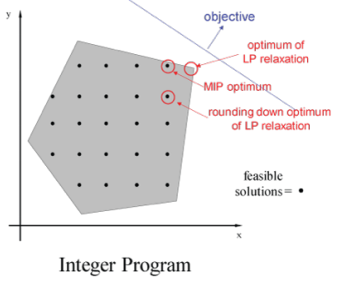
\includegraphics[width=6cm]{integerlinearprogram.png}
\end{tabular}


We can solve this using branch and bounds:

\begin{tabular}{m{12cm}m{6cm}}
    If at the optimal solution of
the linear programming relaxation, one variable is not an integer $x_i =
v$, we create two branches and adding those constraints will only
decrease the upper-bound.
    &
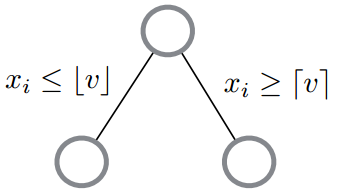
\includegraphics[width=3cm]{branch.png}
\end{tabular}



\subsection{Exam}
\begin{itemize}
    \item Formulate a linear program. 
    \item Be able to transform a LP into standard and slack form. 
    \item Explain and be able to find a initial BFS. 
    \item Apply the simplex algorithm on a small example. (be familiar with the pivoting)
    \item Explain how to detect an unbounded objective.

        $\Rightarrow$ You spot it when you have a var $x_i$ with a
        positive reduced cost in $z$ which always appears in constraints of the form 
        $b_i + x_i = x_n$
\end{itemize}



\section{Lagrangian relaxation}
\subsection{Definition}
The Lagrangian relaxation is a procedure that find a \textbf{lower
bounds}. This
lower bounds will allow to have better performances on the branch and
bounds of the problem starting with an initially good lower-bounds.

\begin{enumerate}
    \item We first relax the problem with the Lagrangian relaxation 
    \item We optimize the $\lambda$ with a sub-gradient algorithm 
    \item We get the optimal $\lambda$ and thus the optimal solution of
        the relaxed problem which is a good lower bounds.
\end{enumerate}

\subsection{Constrained Shortest Path Problem}
In order to represents the concepts discussed in this section, we will
need an example. Lets take the Constrained Shortest Path problem.

\begin{tabular}{m{8cm}m{6cm}}
    \begin{eqnarray*}
        \textrm{minimize } & \sum_{(i,j) \in A} c_{ij} \quad x_{ij} \\
        \textrm{subject to } & \textrm{flow conservation}\\
                            & \sum_{(i,j) \in A } \quad t_{ij} x_{ij} \leq T \\
                             & \forall (i, j) \in A, \quad x_{ij} \in \{0, 1\}
        \end{eqnarray*}

        \begin{itemize}
            \item A example can be to minimize distance with
                \textbf{time constraint} (NP-Hard problem).
        \end{itemize}
& 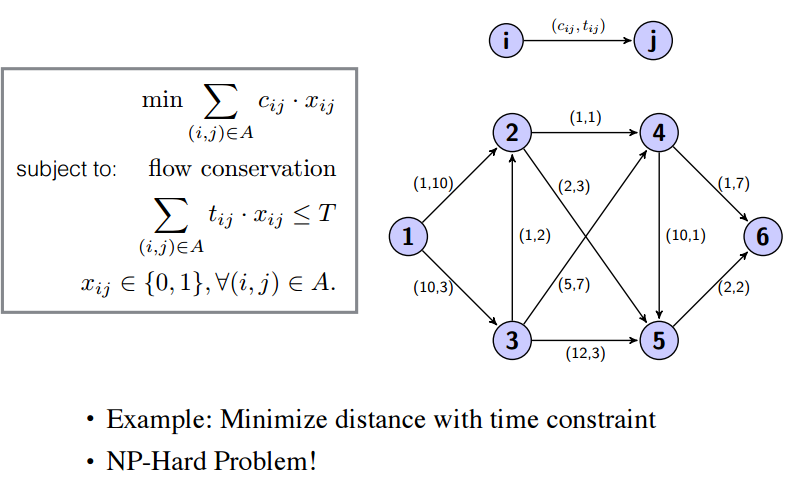
\includegraphics[width=7cm]{lagrangeexample.png}
\end{tabular}


\subsection{Relaxation}

If we remove the resource constraint, the problem is pretty easy. It is
a simple shortest path problem that can be easily resolved with
Dijkstra. What the Lagrangian relaxation does is \textbf{removing the
constraint} and \textbf{adding a new part} in our minimization part.

\begin{eqnarray*}
    L(\lambda) &=& min \sum_{(i,j)\in A} c_{ij} x_{ij} + 
    \textcolor{red}{\lambda \bigg(\sum_{(i,j)\in A} t_{ij} x_{ij} - T
    \bigg)} \\
    &=& min \sum_{(i,j)\in A} \Big(c_{ij} + \lambda t_{ij}\Big) x_{ij} - \lambda T\\
\end{eqnarray*}

$\Rightarrow$ We now have a simple shortest path problem 
where edges has a weight which is a
mixed value of time and distance for a given value of $\lambda$. 

\begin{itemize}
    \item Using this minimization with different $\lambda$ will return
        different solutions. 

    \item Some of them won't be feasibly and will violate the time
        constraint. If you are lucky one of the solution will be the
        optimal one. (hint: try $\lambda = 2$)
\end{itemize}

\subsection{Lagrangian dual}
Now our objective will be to find the best $\lambda$ in order to have
the best feasible solution (the best we can have with Lagrangian, not
necessarily the best of the actual problem, this algorithm is only used
to have a lower bound). We have our Lagrangian dual: 
$$L* = max_{\lambda} \Bigg( min \sum_{(i,j)\in A} (c_{ij} + x_{ij}) -
\lambda \big(\sum_{(i,j)\in A} (t_{ij} x_{ij}) - T\big) \Bigg)$$


\subsection{Find best $\lambda$}

\subsubsection{Brute force}
Formulate the minimization problem as a minimization over the set of all 
the feasible path $\rho \in P$:
$$L* = max_{\lambda} \Bigg( min \{ c_{p} + \lambda\big(t_p - T): \rho
    \in P \}\Bigg)$$

\subsubsection{Sub-gradient algorithm}

\begin{enumerate}
    \item Take an initial $\lambda$ and calculate the solution (Dijkstra resolution)
    \item We check if we are on a 
        \begin{itemize}
            \item increasing edge (violation of the constraint) 
            \item or a decreasing edge (constraint is respected). 
        \end{itemize}

        $\Rightarrow$ Depending of that we will respectively move to
        the right or to the left.
\end{enumerate}

\begin{tabular}{m{9cm}m{9cm}}
    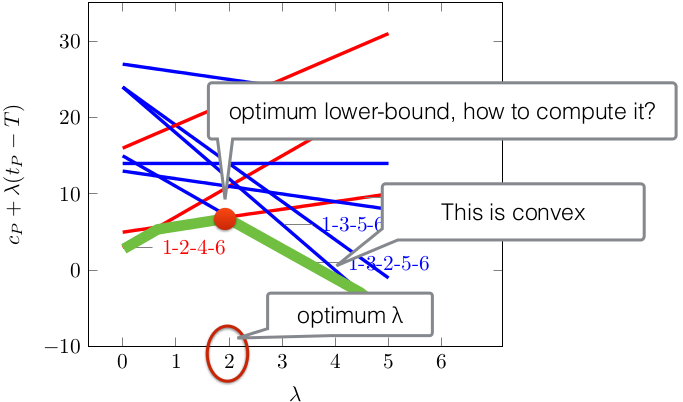
\includegraphics[width=9cm]{lag}
    &
    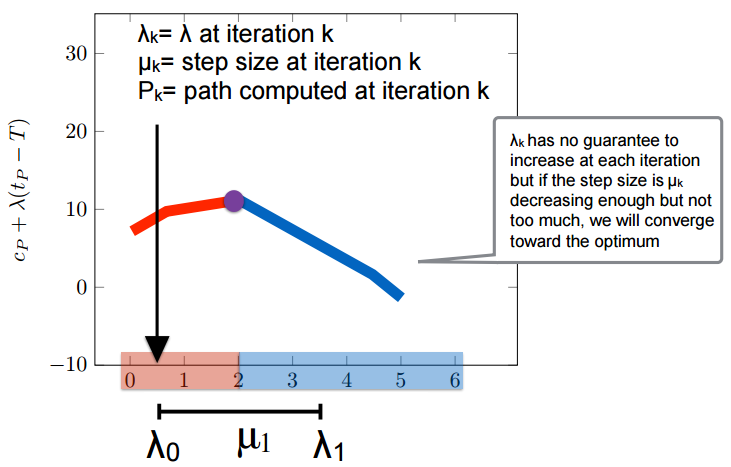
\includegraphics[width=7cm]{lagrangiangraph.png}
\end{tabular}


\begin{itemize}
    \item In order for the algorithm to converge we must reduce the size
        of the step at each iteration. 
    \item It is guaranteed to converge if $\mu_{k} \rightarrow 0$ and
        $\sum^{k}_{j=1} \mu_{k} \rightarrow \infty$.
    \item On the other hand the Lagrangian lower bounds has no
        guaranteed to increase at each step.
    \end{itemize}

\paragraph{Pseudo-code}:

\centerline{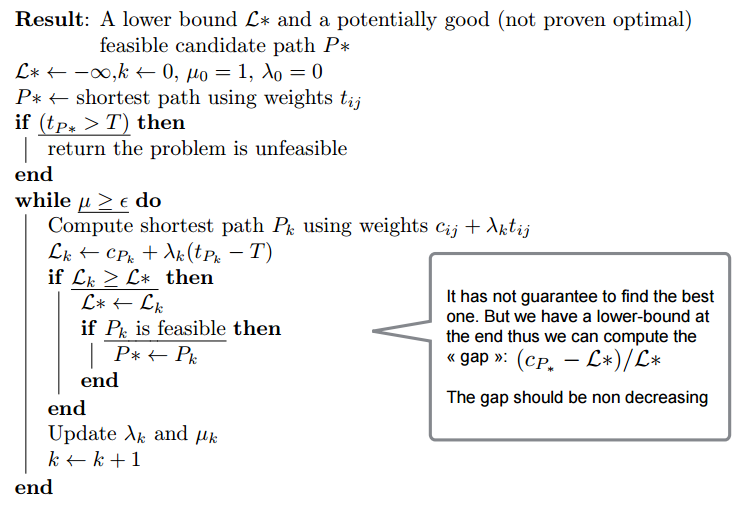
\includegraphics[scale=0.7]{lagrangepseudocode.png}}

\paragraph{Performances}

The Lagrangian relaxation is as good as the linear relaxation. But the
advantage of the Lagrangian one is that it will return feasible solution
during the process.

Typically the lower bounds will evolve along a curve that converge after x steps.

\centerline{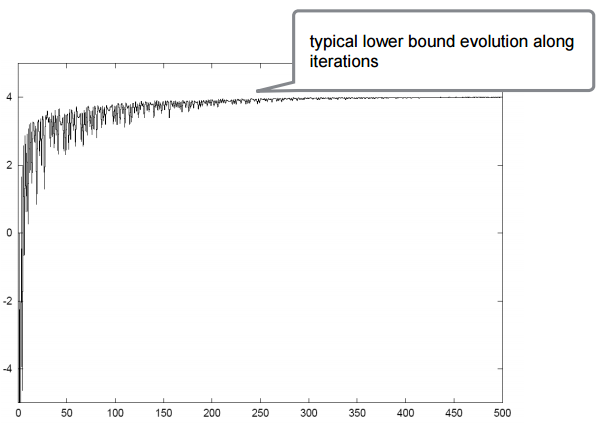
\includegraphics[scale=0.8]{lagrangeconverge.png}}



\section{Network flow}

\subsection{Graph reminder}

\subsubsection{Definitions}

\begin{description}
    \item[A directed graph] is tuple (V, E) where V is the set of vertices 
        and $E \in V x V$ is the set of edges.

    \item[A path] is a suite of distinct nodes $n_0, n_1, ... n_{(k-1)}$ with
        $\big(n_i, n_{(i+1)}\big)$ an
        edge for all $0 \leq i \le k-1$. 

    Node $n_0$ is the origin and node $n_{(k-1)}$ is the
        destination.

    \item[A cycle] is suite of distinct nodes  $n_0, n_1, ... n_{(k-1)}$ with
        $\big(n_i, n_{(i+1)}\% k\big)$ an edge for all $0 \leq i \le k$.
\end{description}

\subsubsection{Graph representation}

\begin{itemize}
    \item Adjacency matrix: The simples one but matrix don't take
        sparsity into account and linear time to iterate over adjacent
        nodes.

    \item Adjacency Lists

        \begin{center}
            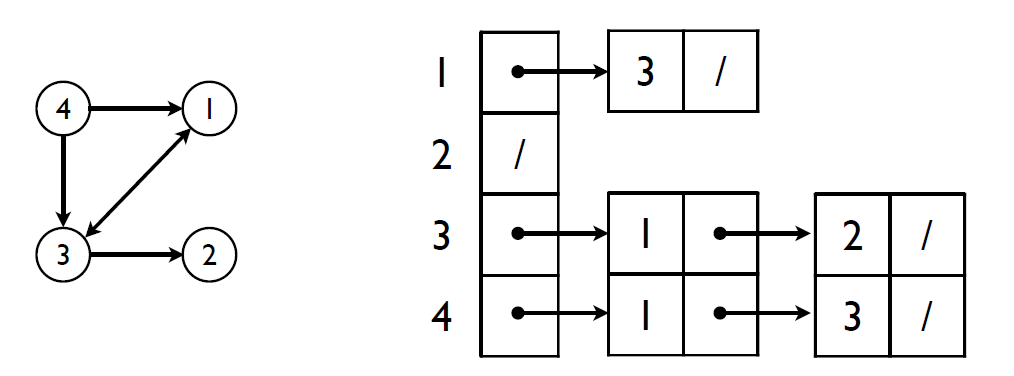
\includegraphics[width=0.3\linewidth]{AdjacencyList.png}
        \end{center}
\end{itemize}


\subsubsection{DFS}

\begin{tabular}{m{6cm}m{6cm}m{3cm}}
    \begin{lstlisting}
DFS(V , E):
    // Initialization;
    Create global variable Color[1..|V |]
    Create global variable P arent[1..|V |]
    for each node $u \in V$ do 
        Color[u] = white
        Parent[u] = Nul
    // Start the search
    for each node $U \in V$ do
        if Color[u] = white then
            Visit(u, V, E)
    \end{lstlisting}
    &
    \begin{lstlisting}
Visit(u, V, E):
    Color[u] = Grey
    for $v \in Adj[u]$ do
        // Explore arc (u, v)
        if Color[v] = white then
            Parent[v] =  u
            Visit(v, V, E)
    Color[u] = black
    \end{lstlisting}
    &
    \begin{itemize}
        \item White: Unvisited
        \item Grey: Not all adjacent edge visited
        \item Black: Fully visited
        \end{itemize}
\end{tabular}

$\Rightarrow$ Say that as we are in a graph, we need to color node that we have
already explored so that we don't reexplore them. 

\paragraph{Complexity}
\begin{itemize}
    \item Init: $O(|V|)$
    \item $O(|V| + |E|)$ : As we have to check every edges at every node
        but we pass on each node once.
\end{itemize}

\subsection{Max flow}

Max flow is a combinatorial problem on Graphs.
He can be solved in polynomial time !

\subsubsection{Definitions}

\begin{itemize}
    \item \textbf{s} is the source and \textbf{t} is the sink
    \item $c(a, b)$ is the \textbf{capacity} between nodes $a$ and $b$.
        ($c(a, b)=0$ if there isn't a edge)

    \item $f(a, b)$ is the \textbf{flow quantity} between node $a$ and
        $b$. (A flow is a vector $f$ such that each composant is associated to a
        pair of nodes.)
$$f(a,b) = -f(a,b)$$ 
\end{itemize}

An \textbf{instance of the Max Flow problem} is characterized by the
graph $G = (V, E)$, the source $s$, the sink $t$ and the vector of
capacity $c$.

\paragraph{Constraints}
\begin{itemize} 
    \item \textbf{Flow conservation} constraint: the
        quantity of water entering into a node (different from
        source and sink) is exactly the same as the quantity of of
        water exiting this node.
        \begin{eqnarray*}
            \forall a\in V\{s,t\} & 
            \sum_{b|(b,a) \in E} \quad f(b,a)  &= \sum_{b|(a,b) \in E}
            \quad f(a,b) 
        \end{eqnarray*}
        Or equivalently
        \begin{eqnarray*}
            \forall a\in V\{s,t\} & 
            \sum_{b \in V} \quad f(a,b)  &= 0
        \end{eqnarray*}

\item \textbf{Capacity} constraint: the flow through each edge does
    not exceed the capacity of this edge.
    \begin{eqnarray*}
        \forall (a,b) \in E & f(a, b) \leq c(a, b)\\
        \forall (a,b) \notin E & f(a, b) \leq 0
    \end{eqnarray*}
\end{itemize}

\paragraph{Flow}
\begin{itemize} 
    \item A \textbf{valid flow} satisfies the two constraints
    \item A \textbf{null} flow is a valid flow where $f(a,b)=0$ for each
        edge
    \item The \textbf{value of a valid flow} is the water quantity out
        of the source. Because of the conservation flow constraint, this
        value is also equal to the quantity entering the sink.
        \begin{eqnarray*}
            v(f) =    \sum_{a \in V |(s,a) \in E} \quad f(s,a)  =
            \sum_{a \in V|(a,t) \in E}
            \quad f(a,t) 
        \end{eqnarray*}

    \item[$\Rightarrow$] The max flow problem is to discover a valid flow of
maximal value
\end{itemize}



\subsubsection{Graphical representation}

\begin{tabular}{m{9cm}m{8cm}}
We usually only represent edges with positive capacity and non
negative flows. We now implicitly add the \textbf{reverse edges} with
capacity 0.
&
    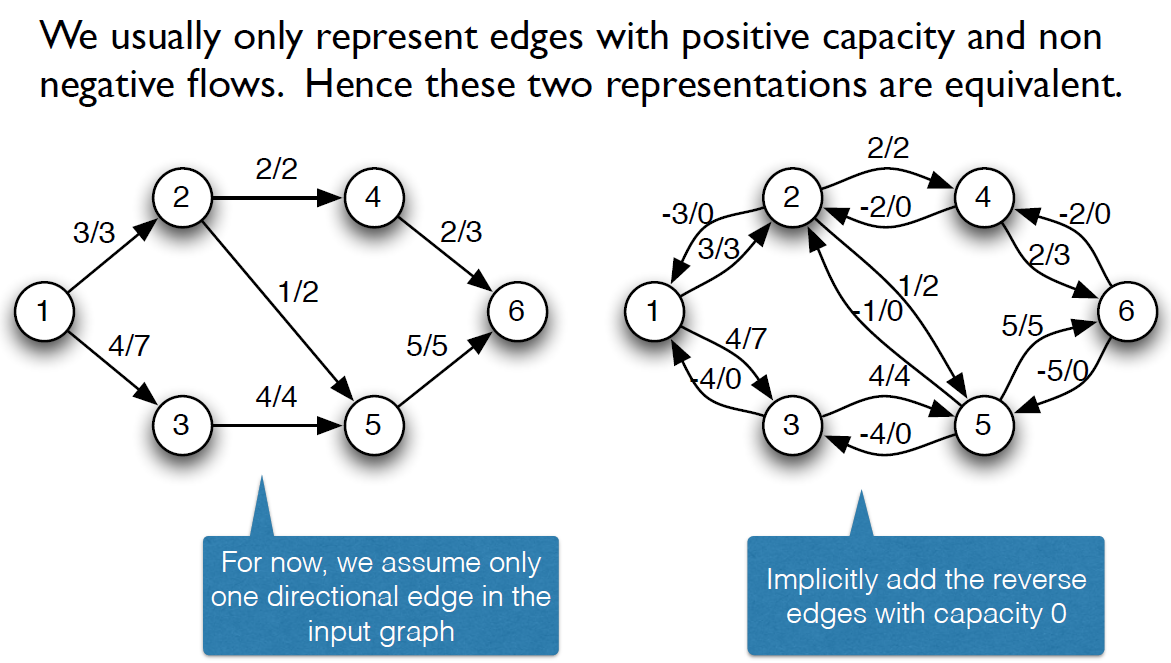
\includegraphics[width=\linewidth]{MaxFlowGraphRepr.png}
\end{tabular}

\begin{tabular}{m{10cm}m{1.5cm}m{1.5cm}}
For bidirectional edges, the reverse edge that we have will have the capacity of the second edge as shown in the example below.
&
    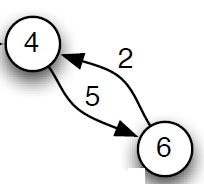
\includegraphics[width=\linewidth]{MaxFlowBidirectionnalRepresentation.png}
    &
    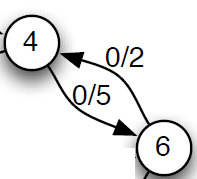
\includegraphics[width=\linewidth]{MaxFlowBidirectionnalRepresentation2.png}
\end{tabular}


\subsubsection{Residual and augmenting path}

\begin{itemize}
    \item \textbf{Residual graph} $G_f = (V, E_f)$ are used to discover paths from the
        source to the sink on which it is possible to push an
        additional quantity of water and so increase the value of the
        flow. 

        \begin{itemize}
            \item This graph is composed of exactly the same nodes as the
                original graph $G = (V, E)$ but the edges may have a different
                direction and a different (residual) capacity.

            \item A edge $(a, b)$ is in the residual only if it is not
                satured (we can add flow):
                $$(a, b) \in E_f \Leftrightarrow f(a, b) < c(a, b)$$

            \item The residual capacity is 
                $$c_f(a, b) = c(a, b) - f(a, b)$$

            \item The residual flow is
                $$f'(a, b) = \begin{cases}
                    f(a,b) + q & if (a, b) \in C\\
                    f(a,b) - q & if (b, a) \in C\\
                    f(a,b)  & otherwise\\
                \end{cases}$$
        \end{itemize}

        \begin{center}
            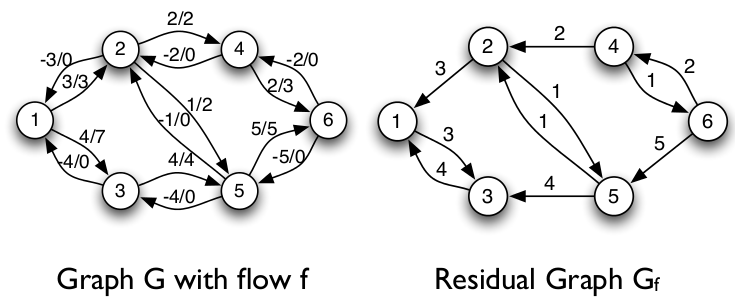
\includegraphics[width=8cm]{residualGraphExample}
            \end{center}

    \item A path joining the source $s$ to the sink $t$ in the residual
        graph $G_f$ is called \textbf{augmenting path}.
\end{itemize}


\subsubsection{Ford-Fulkerson Algorithm}

\begin{lstlisting}[mathescape]
Ford-Fulkerson(V, E, c, s, t):
// Build a vector $f$ with $\frac{|V|}{2}$ entries initialized at 0
    do
        Build the residual graph $G_f$ 
        Find a path $C$ from $s$ to $t$ in $G_f$ 
        if such a path exists then
            Let q be the smallest residual capacity on an edge of path C;
            for every edges $(a, b)$ of path $C$ do
                $f (a, b) = f (a, b) + q$
                $f (b, a) = f (b, a) q$
    while we cannot find a path between $s$ and $t$ in $G_f$ 
    return $f$ ;
\end{lstlisting}

\subsubsection{Complexity}
As the complexity of the algorithm is $O(|V| |E| U)$ with U the
maximum flow of the graph. The complexity is thus not polynomial but
pseudo-polynomial (because the input takes $log(U)$ bits to represent
$U$). For this algorithm to be polynomial you must use
delta scaling.

%TODO: sure about pseudo-code
\begin{lstlisting}
Delta-Scaling :
    delta = X > 1
    while true {
        Filter out all edges with capa < X in residual graph
        if you find an augmenting path :
            delta *= 2
            q = smallest capa of path
            for every edge of path do:
                f(a,b) = f(a,b) + q
                f(b,a) = f(b,a) - q
        else if delta > 1 :
            delta /= 2
        else
            break;
    }
    return result
\end{lstlisting}


As their are a maximum of log(U) iteration with delta scaling, the
algorithm is of polynomial complexity. The complexity becomes 
$O(|E|^2 log U)$

\begin{figure}[!ht]
    \centering
    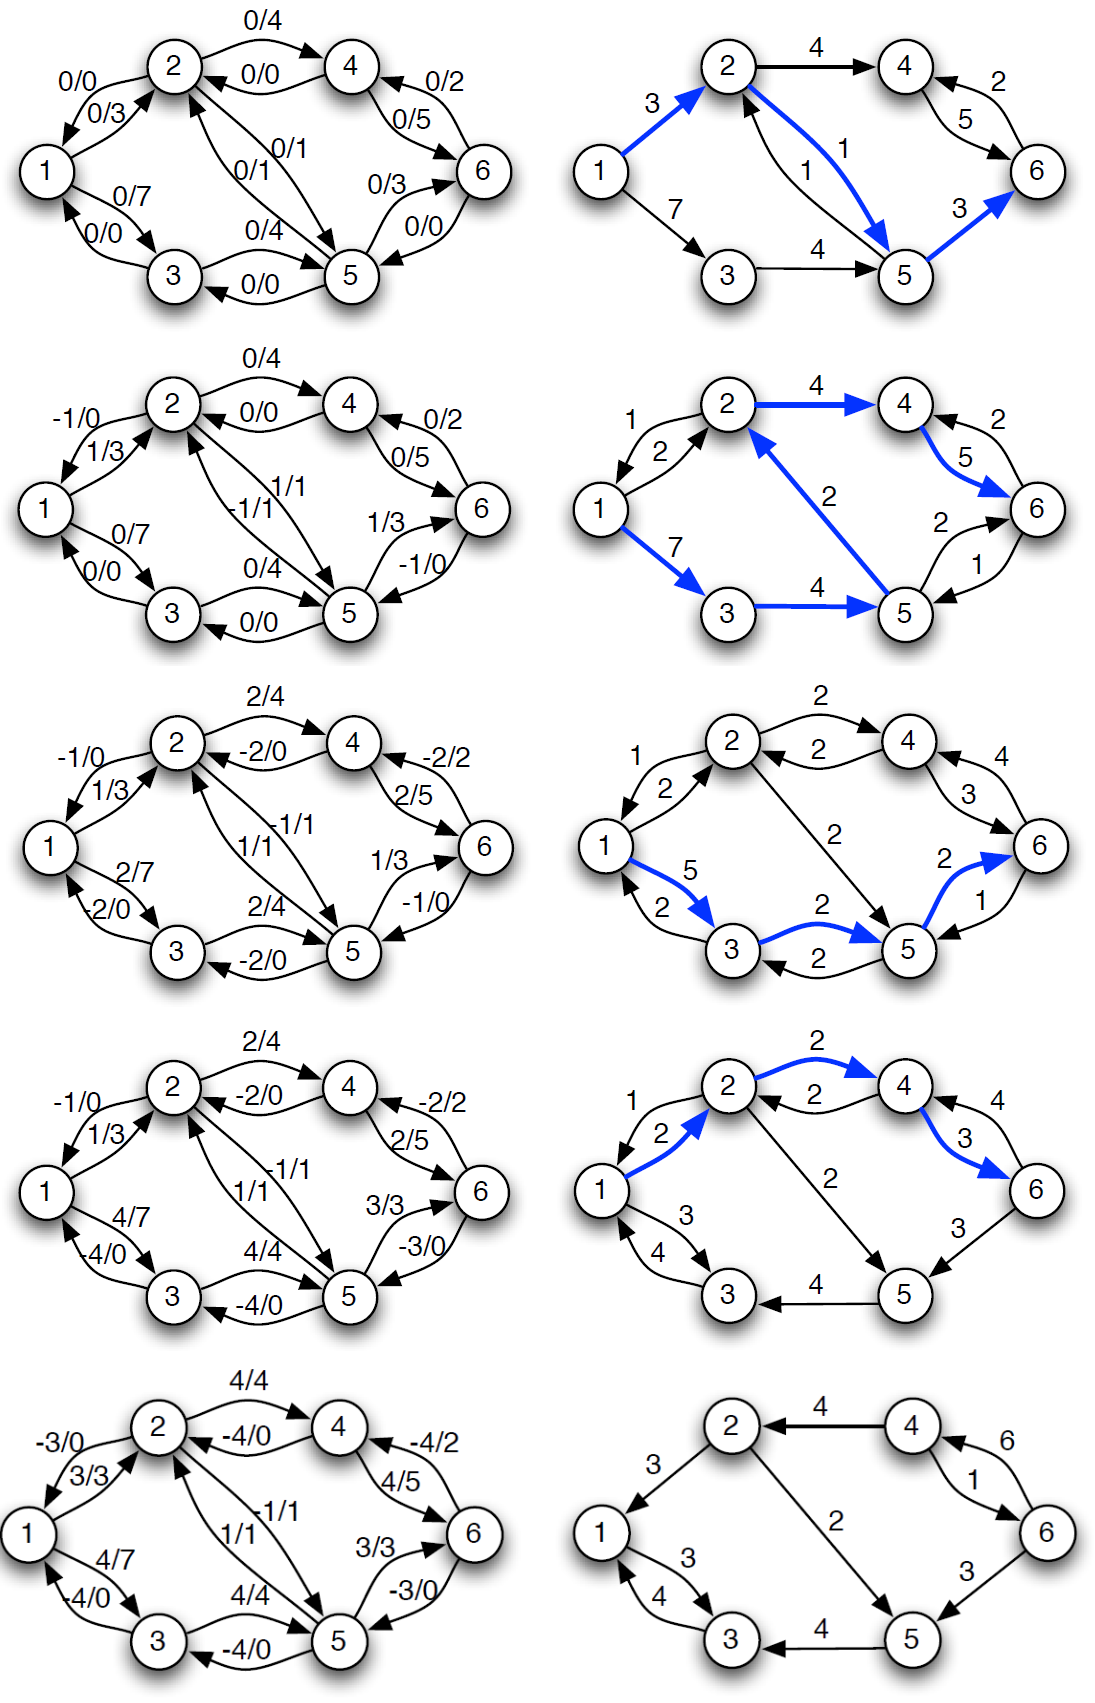
\includegraphics[width=0.55\linewidth]{MaxFlowAlgoExecutionExample.png}
    \caption{Ford-Fulkerson runtime example}
    \label{fig:Ford-Fulkerson_example}
\end{figure}


\subsection{Min cut}

How much cut do we have to make to partition a graph such that two node
$s$ and $t$, are in different partition. Answer == MaxFlow(s,t)

\subsubsection{Definitions}

\begin{itemize}
    \item A cut is bipartition of a set V formed of two disjoint sets
        $S$ and $T$ such that $V$ is the union of $S$ and $T$.
        $$S \cup T = V \quad \quad S \cap T = \emptyset $$

    \item A cut in a network is a bipartition ($S, T$) of the nodes such
        that the source is in the set $S$ and the sink is in the set $T$
        $$S \cup T = V , s\in S\quad \quad S \cap T = \emptyset, t \in
        T$$

    \item The capacity of a cut (S, T) is the capacity of the edges
        linking
        a node from S to a node in T.
        $$c(S, T) = \sum_{a\in S} \sum_{b \in T} c(a, b)$$

    \item The net flow of a cut ($S, T$) is the quantity of flow
        (positive or
        negative) from a node in S to a node in T.
        $$f(S, T) = \sum_{a\in S, b\in T} f(a, b)$$

\end{itemize}

\paragraph{Example}

        \begin{tabular}{m{5cm}m{6cm}}
            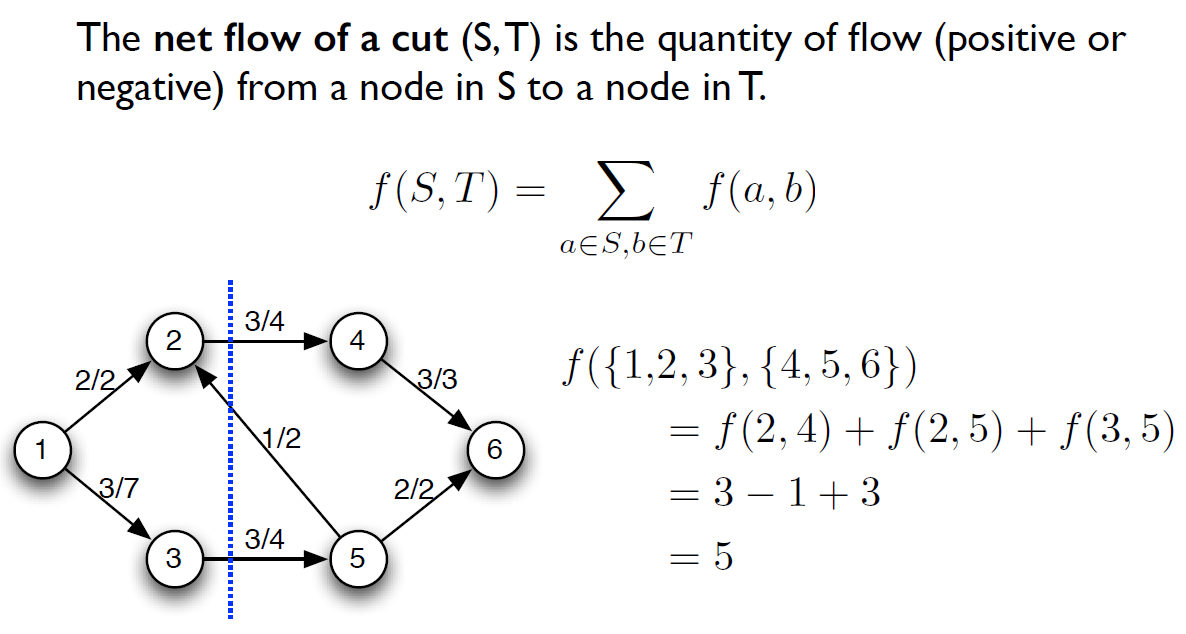
\includegraphics[width=\linewidth]{CutDefinition1.png}
            &
                \begin{eqnarray*}
                    c(\{1, 2, 3\}, \{4, 5, 6\}) & =& 8\\
                        \\
                        f(\{1,2, 3\}, \{4, 5, 6\}) & =& f(2, 4) +
                        f(2, 5) + f(3, 5)\\
                        & =& 3 - 1 + 3 \\
                        & =& 5
                    \end{eqnarray*}
        \end{tabular}


\subsubsection{}
\begin{center}
    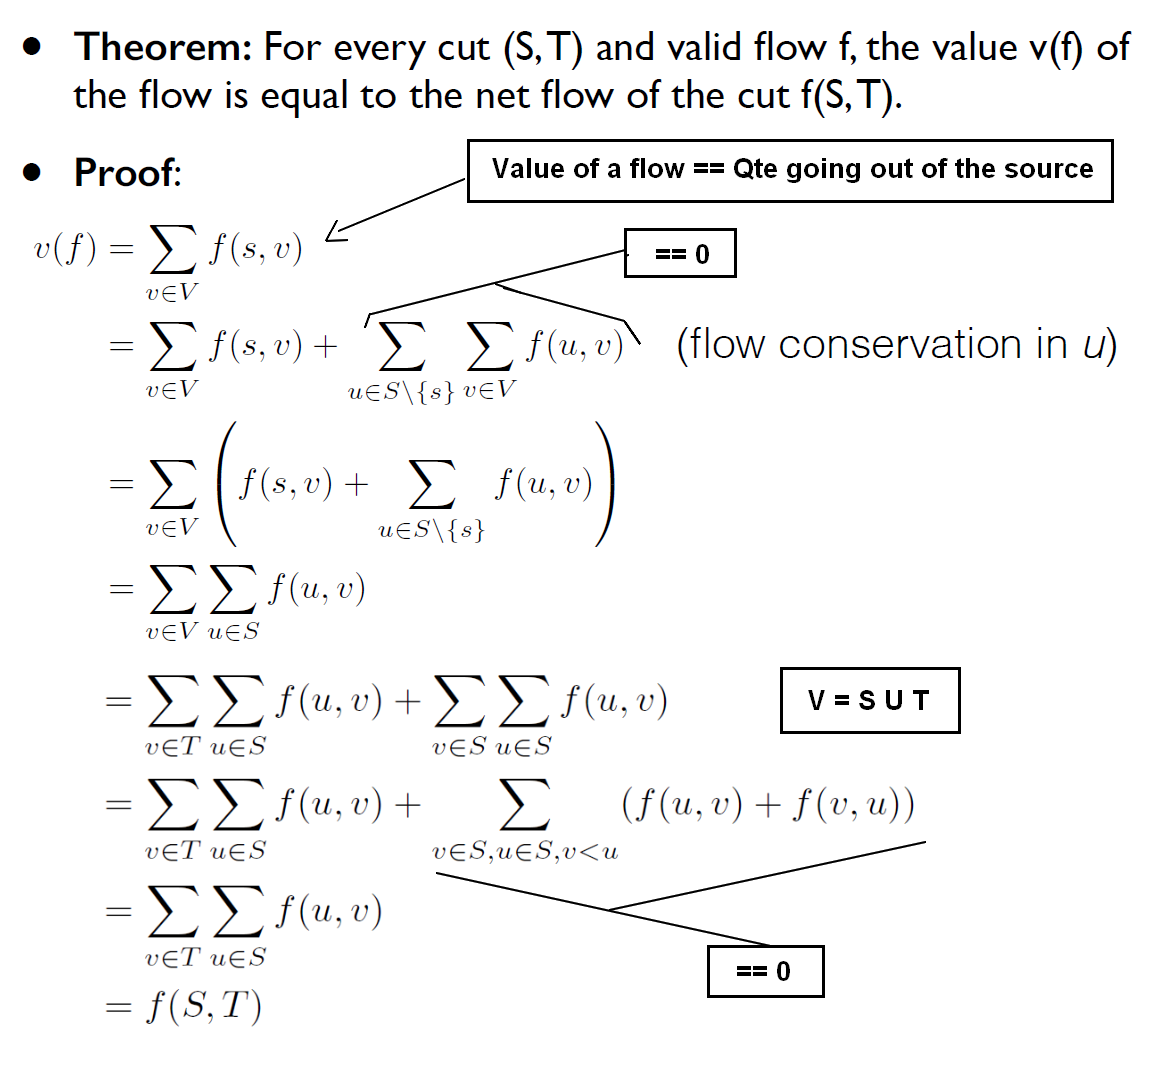
\includegraphics[width=0.7\linewidth]{CutProof.png}
\end{center}

\subsubsection{Proof that min cut is solved by max flow}
\subsection{Max flow - min cut theorem}
Given a feasible flow f, these properties are equivalent:
\begin{enumerate}
    \item f is maximum flow in G;
    \item The residual graph G f has no augmenting path
    \item There exists a cut (S, T) with capacity c(S, T) equal to
        v(f).
\end{enumerate}

\subsubsection{}
For any feasible flow f of value v(f), there exists a cut (S,T) such
that the flow f(S,T) that crosses the cut is equal to v(f). Since for
any feasible flow we have f(S,T) <= c(S,T), if you find a flow v(f) =
f(S,T) = c(S,T), then you can't find a cut with capacity less than
c(S,T) (the flow v(f) would still have to pass through the cut because
it's a valid flow). Hence any cut with v(f) = c(S,T) is minimal.

\subsection{Min cost flow}
\begin{enumerate}
    \item Start with a flow of zero
    \item  Find an s-t path in G f with minimum weight
    \item  Augment along this path as much as possible (limited by
        smallest
        residual capacity of the path).
    \item  Repeat two previous steps until initial demand B of the source
        is met.
\end{enumerate}

\begin{figure}[!ht]
    \centering
    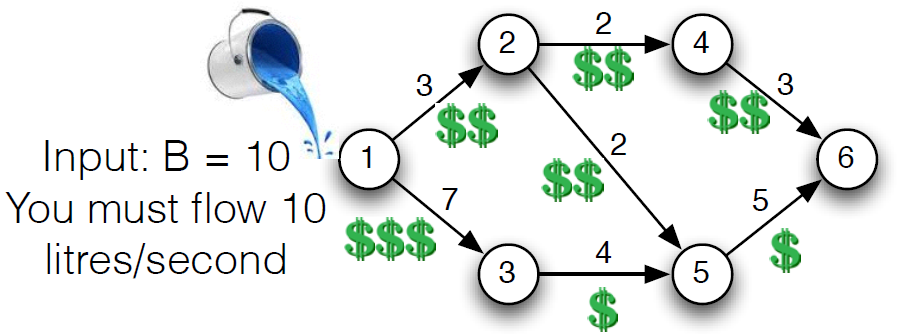
\includegraphics[width=0.5\linewidth]{minFlow.png}
\end{figure}

Be careful that in some problem negative weight may be used and infinite
loop must thus be avoided. => Use the Moore-Bellman-Ford algorithm
\url{https://en.wikipedia.org/wiki/Bellman%E2%80%93Ford_algorithm} 



\subsection{Scheduling}

\begin{tabular}{m{8cm}m{7cm}}
4 persons must give a seminar in a
single room with their possible slots.
\begin{itemize}
    \item  Alice (11h, 13h); Benoit (9h, 10h, 13h);
        Clotilde (9h, 11h, 13h) and Dany (11h, 13h).
\end{itemize}
&
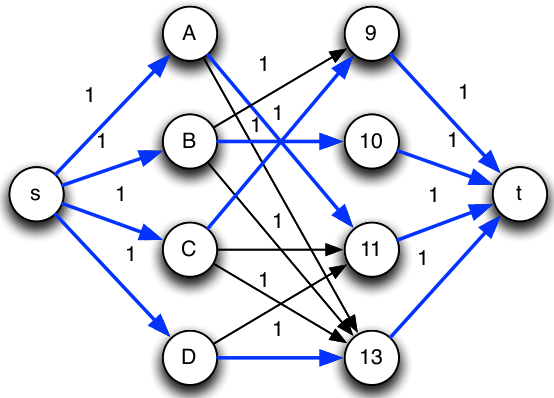
\includegraphics[width=6cm]{flowSchedul.png}
\end{tabular}






\section{Greedy and approximation algorithms}

\section{Greedy and approximation algorithms}


\subsection{An activity-selection problem}
\begin{tabular}{m{6cm}m{10cm}}
    Find the max number of activities that do not
    overlap in time : 
    $$\forall i,j \quad selected: \quad s_i \geq f_j  \quad or \quad s_j \geq f_i$$
    &
\begin{itemize}
    \item $s_i$ = start time of activity
    \item $f_i$ = end time activity (not that activities are 
        sorted such that $f_i \leq f_{i+1}$)
\end{itemize}
\end{tabular}

\begin{enumerate}
    \item \textbf{Reduction} to the maximum independent set problem where 
        we find the maximum set of vertices in a graph such that
        to vertices selected are not adjacent.

        \begin{tabular}{m{10cm}m{3cm}}
            \begin{itemize}
                \item The reduction is done by add an edge between $i$ and $j$ if
                    activities overlap in time: 
                    $$s_i < f_j and s_j < f_i$$ 
            \end{itemize}
            Note that the maximum independent set problem is NP-Hard problem
            &
            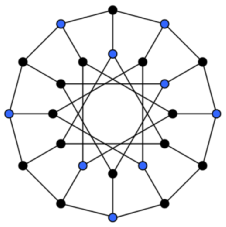
\includegraphics[width=3cm]{img/independant}
        \end{tabular}


    \item \textbf{Dynamic programming}: select a maximum size subset of mutually
        compatible activities from $S_{ij}$, for $0 \leq i < j \leq n+1$,
        knowing that all other $S_{ij}$ are empty.

        $a_m$ such that $f_m = min\{f_k: a_k \in S_{ij}\}$
        \[
            c[i, j] = 
            \begin{cases} 
                0 & \text{if } S_{ij} = \emptyset \\
                max_{\substack{i<k<j \\ a_k \in S_{ij}}} \{c[i, k] + c[k, j] + 1\}  & \text{if } S_{ij} \neq \emptyset
            \end{cases}
        \]
        \begin{itemize}
                %TODO
            \item Time complexity: 
            \item Space complexity: 
        \end{itemize}

        \paragraph{Improvement to a greedy}
        \begin{itemize}
            \item Obs.1: a m is used in some maximum-size subset of
                mutually compatible activities of $S_ij$

                Proof (Sketch):
                \begin{small}
                    Suppose $A_{ij}$ an optimal set of $S_{ij}$ . Take
                    the first activity of $A_{ij}$ (assume it is $a_k$ with $k \neq m$). We
                    can safely replace $a_k$ with $a_m$ because $f_m \leq f_k$.
                \end{small}

            \item Obs.2: The subproblem $S_im$ is empty, so that choosing
                $a_m$ (in the recurrence) leaves the subproblem $S_mj$ as the
                only one that may be nonempty.
        \end{itemize}

        %TODO new recurrence equation

    \item \textbf{Greedy algorithm}
        \begin{lstlisting}[mathescape]
n $=$ nbrActivities
A $= a_1$
i $= 1$

for m $\leftarrow$ 2 to n do
if $s_m \geq f_i$ then
A = $A \cup a_m$
i =$m$

return A
        \end{lstlisting}
\end{enumerate}


\subsection{Greedy}
At each decision point, the algorithm makes
a \textbf{local optimum choice} in the hope that it is a global
optimum choice.
\begin{itemize}
    \item For some problem it's the case
    \item For other it's not and sometimes we can 
        have a guarantee how
        \textit{suboptimal} we can be.
\end{itemize}


\subsection{Minimum Spanning Tree (MST)}

\subsubsection{Definition}
\begin{itemize}
    \item A \textbf{cut} (S,V-S) of an undirected graph
    \item An edge (u,v) \textbf{cross} the cut (S,V-S) if one of its
        endpoints is in S and the other in V-S
    \item A cut \textbf{respects} a set A of edges if no edge in A crosses
        the cut.
    \item An edge is a \textbf{light edge} crossing a cut if its weight is
        the minimum of any edge crossing the cut. (can be
        more than one in case of ties).
\end{itemize}

\subsubsection{Theorem}
\begin{itemize}
    \item[LET]
    \item $G=(V,E)$ a undirected graph with weight function $w$ on $E$.
    \item $A \subseteq E$ included in some MST for $G$.
    \item $(S, V-S)$ be any cut of $G$ that respect $A$
    \item $(u,v)$ be a light edge crossing $(S, V-S)$
    \item[THEN]
    \item edge $(u, v)$ is safe for $A$
    \end{itemize}

\subsubsection{Algorithm}

\begin{lstlisting}[mathescape, caption=Generic-MST(V\,E\,c\,s\,t)]
A = $\emptyset$
while A does not form a spanning tree do
    find an edge $(u, v)$ that is safe for A
    A = A $\cup \{(u, v)\}$

return A
\end{lstlisting}

\begin{itemize}
    \item \textbf{Kruskal} 

    \item \textbf{Prim} 
\end{itemize}

\subsection{Exam}
\begin{itemize}
    \item All theoretical notions introduced (proofs, etc).
    \item Design a greedy algorithm
    \item MST: I give you a new MST greedy algorithm. You
        should be able argument whether it is correct or not.
    \item Design a simple approximation scheme, compute it’s
        approximation ratio
    \item I give you a complexity of an approximation scheme.
        You should be able to tel me if it is fully polynomial.
\end{itemize}



\section{Local search}

\subsection{Generic Local Search}
1) An initial solution s\newline
2) N(s) is the neighborhood of s\newline
3) Some moves are legal (satisfy the constrains) some arn't : L(N(s),s) is the set of legal moves from a solution s.\newline
4) S selects the move in the legal moves


\begin{figure}[!ht]
    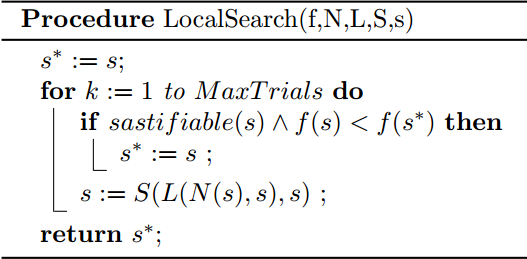
\includegraphics[width=0.4\linewidth]{LocalSearchGenericAlgo.png}
    \label{fig:Knapsack_example}
\end{figure}
\FloatBarrier
 

\subsection{Improvement Heuristic}
We can improve this algorithm with two heuristics:\newline
\textbf{L-Improvement} will only accept moves that improve the solution\newline
\textbf{S-Best} will select one on the move randomely in case of tie.\newline

\subsection{Local Minima}

A big problem with local search is that you can be stuck in a local minima(maxima) for a minimization problem(maximimzation).\newline

We have two solutions for that:\newline
1)We can accept to degrade the solution\newline
2)Enlarge the neighborhood\newline

\subsection{Sudoku exemple}
There is two type of constraints : Hard and Soft.\newline
\textbf{Hard Constraints} much be respected at all time during the local search.(They are enforced at initialization)
\textbf{Soft Contstraints} are the constraints that can be violated during the search in order  to find better solutions.\newline

For the sudoku exemple we execute swaps between cases to try to lower the number of soft constraints violated.

Adding more constraints in the hard constrains makes the initialization harder but makes the local search process easier.

\subsection{OscarR CBLS}
\textbf{OscarR CBLS} is a library for local search.
You add the constraints and the objectifs function and it will compute the violations and the delta's for you.

With this you can focus more on the search process(moves and meta-heuristics).

\subsection{Tabu Meta Heuristic}
\textbf{Tabu meta heuristic} accept to degrade the solution in order to get out of the local minimas.\newline

Whenever you perform a move, this move becomes tabu for a certain duration(number of iteration).When you are stuck in a local minima the algrithm keeps iterating between a couple of moves without finding a better solution. By making a move tabu you force it to chose some other point and escape from the  local minima.\newline

If your neightboord is connected and you let the tabu search run indefinatly with a long enought tabu periode your algorithm will end up finding the optimal solution

\subsubsection{Improvement on tabu search}
Aspiration\newline
You not only consider the non tabu moves but you also considere the best tabu moves if they improve your best solution.
You might have use a certain move to get out of a minima at some point and escape from this local minima. But after that maybe the move is still tabu but alows you to find a better solution that the one you have found so far. Aspiration allows you to find this better solution even tought the move is in the tabu list.

Restart\newline
Every X iteration you change randomely some variables in you current solution and you restart the from that point. This allows you to travel further in the search space in order to maybe find a better solution far from the position you were before.

\subsection{Connected Neighborhood}
A neighborhood is connected if and only if for each
solution s, there exists a path to an optimal solution s*.

This means that if you make the right moves, your neighboord is large enought to find the optimal solution. However having a connected neighboord doens't means you will find the optimal solution(in case you don't make the right moves because of a bad heuristic for instance).\newline

with a connected Neightboord you are not forced to restart(even thought this can improve the time to find the best solution).
Also you can find the solution find a random heuristic.

\subsection{Lin-Kernighan algorithm}
In a TSP, 2-opt is an algorithm that swap 2 edges.
3-opt is the algorithm that swap 3 edges, 4-opt..
Obviouly there is more 3 opt moves than 2 opt move and more 4 opt moves than 3 opt moves...
Above a 4-opt the neighboord is getting way too big.
This is why we can limit ourself to \textbf{Sequential k-Opt moves}.
A k-Opt move is called sequential if it can be described
by a path alternating between deleted and added
edges.

We want to greedily build a Kk-opt move(maybe not THE best move in the k-opt neighboord).
We will start this algorithm with different k's and use the one that gives use to most gain.

This algorithm is the Lin-Kernighan.
We build a set X and Y of edges such that X are the deleted edges and Y are the added edges
Those edges are added elements by elements(empty at start).
We could start the algirthm just like that but we don't want it to run forever. This is why we add some criteria to make is sufficiently efficient.\newline

The sequential exchange criterion\newline
There can not be two added edges in a row. There must be an added edge folowed by a deleted edge.
The feasibility criterion\newline
The resulting configuration must be a cycle.
The positive gain criterion\newline
We chose the set Y of edge so that we gain from the nex configuration(If the changes gives us a worst solution than the one we had before it is not interresting)
The disjunctivity criterion\newline
X and Y disjoint(You can't add a deleted edge or you can't delete an added edge.
The candidate set criterion\newline
When looking for a new edge in Y we limit ourself to only considere the 5 nearest neighbors of the vertice.\newline

\subsection{ATSP reduction to TSP}
ATSP = Asymetric traveler salesman problem.
This means that the weight of the edge from A to B isn't neceseraly the same as the one from B to A. To reduce this problem to the simple TSP we double every every vertice and put an -inf weight to it.\newline

\subsection{Vehicule Routing Problem}
This a local search problem mixing the bin packing problem and the TSP problem.
We have two types of initializations for this local search.\newline
\subsubsection{Saving Heuristics}
We start with a single vehicule for each customer we need to serve.
Afterthat we merge routes to decresae the total distance the most without exceeding the capacity.We do that iteratively until no more routes can be merge withtout violating the capa constraints\newline

\subsubsection{Sweep Heuristic}
Westart with a ray centered at the depot.We start the turn the ray around the depot and every time we cross a customer with the ray we add it to the current cluster. If the nest customer exceed the capacity we start a new cluster.\newline

\subsection{Scheduling moves}
We have a set of activities that can not be interrupted and that have a certain length and a certain ressource need.
The ressource capacity is C.
How to minimize the total duration withtou exceeding the total capcity.\newline
We can use the IFlat-IRelax algorithm(Local search algorithm).\newline
We iterativelay flatten then Relax.\newline
1)\textbf{Flatten} : We add strong percedences constraints until the capcity constrains is satisfied.
2)\textbf{Relax} : We remove some precedences randomely on the critical path(the critical path is that path that is the longest in the schedule(the one that makes the schedule the longer)

\subsection{Eternity II}
16x16 edge matching puzzle.\newline
What neightborhood should we chose?\newline
Remove m pieces from non edge adjacent positions(up to $n^2/2$ ) and remplace them optimally. \newline
Exemple : We remove 5 edges and check for every single on of those pieces the number of correct adjacent edges it gives us. We have a complete weighted bipartite graph beteen the removed piecs and holes that we can solve thanks to a maximum assignement problem.
The size of the Neighborhood is exponential but it can be optimally explored in polynomial time.(Hungarian algorithm O(m³).



\section{Constraint programming}

\begin{itemize}
    \item \textsc{Model} : Describe real world problem with
        \begin{itemize}
            \item \textbf{Variables} : $X = \{x_1, x_2,\cdots, x_n\}$

            \item \textbf{Domains} : $D = \{ D(x_1), D(x_2),\cdots,
                D(x_n)\}$

                \begin{itemize}
                    \item[Ex:] Booleans, \textbf{finite domains}, finite
                        set, intervals, continuous domains,\ldots
                \end{itemize}
            \item \textbf{Constraints} : $C = \{c_1, c_2,\cdots, c_e\}$
                \begin{itemize}
                    \item A \textbf{scope} $\scp(c) = (x_1, x_2,\cdots,x_{r_e})$ : is the
                        variables constrained by c.
                    \item A \textbf{relation} $\rel(c)$ : value combinations accepted by
                        c
                \end{itemize}

                \begin{tabular}{m{1.5cm}m{12cm}}
                    Used for:&
                \begin{enumerate}
                    \item Feasibility checking: Check if the constraint can be satisfied
                        given it's variables domain. 

                    \item Pruning: remove values from the domains if they do not appear
                        in any solution of the constraint.
                \end{enumerate}
                \end{tabular}

            \item \textbf{Objective function} : $O : \sol \to \R$
        \end{itemize}

        \paragraph{Types}
        \begin{enumerate}
            \item CSP${} = (X, D, C)$
            \item COP${} = (X, D, C, O)$
        \end{enumerate}

        \paragraph{Declarative} : describe what you want not how to get it

    \item \textsc{Search} : Describe how to solve the problem and
        explore the search space
        \begin{itemize}
            \item \textbf{Propagation} : Use constraints to remove
                \textit{useless} (doesn't remove solution) parts of the
                search space. It's a filtering where we remove
                value from non feasible solutions.
                \begin{center}
                    \scriptsize
                    \textit{Need choice between more pruning with more
                        expensive to compute or less proning cheaper to
                    compute}
                \end{center}

                \begin{itemize}
                    \item Consistencies : Require that all the values
                        are able to satisfy their constaints in
                        \textbf{isolation}

                    \item Propagator: used at the beginning of the search
                        and each time a decision is made.
                \end{itemize}
            \item \textbf{Backtracking Tree Search} : Explore search
                space by taking decisions and backtracking (with
                remembering decision)

                \paragraph{Current node}: The node is modified at each decision
                made and it is restored when backtracking occurs.
        \end{itemize}

        \paragraph{Search space} = $D(x_1) \times D(x_2) \times \cdots \times D(x_n)$
\end{itemize}

The communication between the Constraints and the Search is done through the domain of the variables in CP.
When a constraint modify the domain, it is called \emph{propagation} and when it is the search it is called \emph{branching}.


\subsection{Pruning}

\subsubsection{Fix-point algorithm}

\begin{lstlisting}
repeat
    select a constraint c
    if c is OK wrt the domain store
        apply pruning algorithm of c
    else
        return KO
until no value can be removed
\end{lstlisting}

\begin{tabular}{m{8cm}cm{8cm}}
    %TODO tikz
    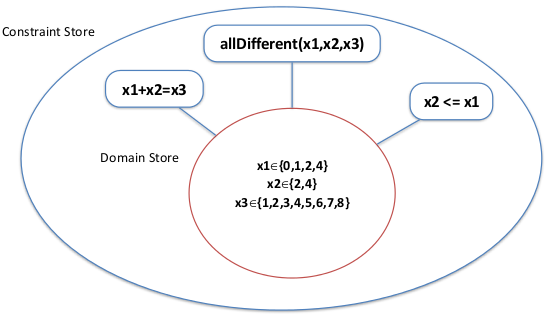
\includegraphics[width=8cm]{fixPoint1}
    & $\Rightarrow$ &
    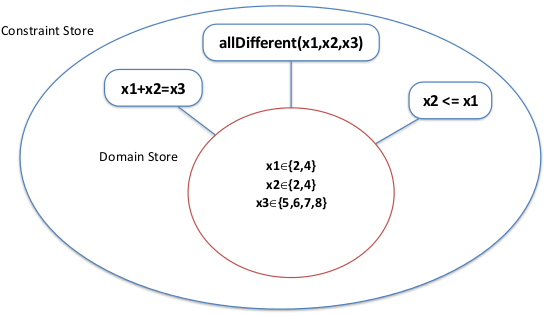
\includegraphics[width=8cm]{fixPoint2}
\end{tabular}


\subsection{Consistency}

\begin{itemize}
    \item A CSP (\textsc{X, D, C}) is $X_{Consistent}$ iff all
        constraints $c \in C$ are $X_{Consistent}$ ($X_{Consistent}$ is
        GAC, BC,\ldots)

    \item A consistency $S_1$ is stronger than a consistency $S_2$ iff all CSP respecting
        $S_1$ also respect $S_2$.

        Note that some consistencies can be \textit{incomparable}

        \begin{center}
            \begin{tabular}{l|c|c|}
                \cline{2-3}
                \multirow{1}{*}{
                    \begin{tikzpicture}
                        \node (0,0) {};
                        \draw[->] (0,1.5) edge node [left]{\rotatebox{90}{Strongest}}
                        (0, 2.5);
                \end{tikzpicture}} 
                &
                \multicolumn{2}{c|}{GAC} \\
                \cline{2-3}
                & Bound consistency & Forward checking \\
                \cline{2-3}
            \end{tabular}
        \end{center}

        This is a tradeoff between \textbf{Speed} and \textbf{Filtering}.

\end{itemize}


\subsubsection{Filtering consistencies}

if $x$ is a domain filtering consistency, a propagator for $x$ will :
from CSP(X, D, X)
\begin{itemize}
    \item return (X, D', C) such that
        \begin{itemize}
            \item D' $\subseteq$ D
            \item (X, D, C) and (X, D', C) equivalent
            \item D' is a nonempty partial solution
            \item (X, D', C) respect $x$
        \end{itemize}
    \item return \textcolor{red}{fail} if no such CSP exists.

        $\to$ not possible to satisfy consistency = unsatisfiable CSP
\end{itemize}

\begin{itemize}
    \item \textbf{Arc consistency} (also called domain consistency):
        every value of every variable participates in a solution of the
        constraint, so all value of variables are \textbf{supported}.

        \begin{tabular}{m{1cm}m{13cm}}
            Note:&
        \begin{itemize}
            \item It's the strongest filtering when considering constraints in isolation.
                \item  GAC $\neq$ satisifability :i A CSP that is GAC may not
        be satisfiable.
        \end{itemize}
        \end{tabular}

        \paragraph{GAC} A constraint $c$ is GAC iff
        \begin{lstlisting}[mathescape]
$\forall x_i \in scope(c)$
    $\forall a_i \in D(x_i)$
        $\exists a_1,..., a_{i-1}, a_{i+1},..., a_r \in D(x_1) \times ... \times D(x_{i-1}) \times D(x_{i+1}) \times ... \times D(x_r)$ such that $(a_1,...,a_r) \in c$
        \end{lstlisting}


    \item \textbf{Bound consistency}: assuming domains are intervals,
        every bound of every variable participates in a solution of the
        constraint.

        \begin{itemize}
            \item GAC can be costly, so a other consistency is to
                only search support for bound.
            \item[$\to$] all valuyes between min and max considered in the domain.
        \end{itemize}


        \paragraph{BC} A constraint $c$ is BC iff
        \begin{lstlisting}[mathescape]
$\forall x_i \in scope(c)$
    $\forall a_i \in \{ \quad min(D(x_i)), max(D(x_i))\quad \}$
        $\exists a_1,..., a_{i-1}, a_{i+1},..., a_r  \in D*(x_1) \times ... \times D*(x_{i-1}) \times D*(x_{i+1}) \times ... \times D*(x_r):$ such that $c(a_1,..., a_r)$

$D*(x_k) = [min(D(x_k)), max(D(x_k))]$
        \end{lstlisting}


    \item \textbf{Forward checking}

        It's like a GAC at the end.

        \paragraph{FC} A constraint $c$ is FC iff
        \begin{lstlisting}[mathescape]
if $\forall x_i \in scope(c):$ $D(x_i) = \{v_i\}$ then $c(v_1, ..., v_r)$
if all but one variable assigned: $c$ is GAC
        \end{lstlisting}
\end{itemize}



\subsection{Global constraints}

\paragraph{Advantage}
\begin{itemize}
    \item Increasing expressivity of CP
    \item Pruning strength because the propagation considered constraint in isolation
        but global constraint is like \textbf{a set of constraint}
    \item Pruning efficiency because no fixed point between small constraints
        but a more flobal reasoning
\end{itemize}

\subsubsection{Decomposition}
A set of constraints $S$ is called the decomposition of $g$ iff :
$$ \forall D(X): sols(X, D(X), \{g\}) = sols(X, D(X), S)$$

\begin{itemize}
\item GAC pruning equivalent in $S$ and $g$ iff the constraint
graph of the D is \textbf{acyclic}.

Otherwise, GAC pruning stronger in global constraint

\begin{itemize}
    \item GAC on decomposition : supports(s) for each literal on each constraints
        \textbf{separately}
    \item GAC on global constraint: global support(s) for each literal on global constraint
\end{itemize}


\item FC pruning stronger in the decomposition
    \end{itemize}



\subsubsection{AllDifferent constraint}

GAC pruning for \texttt{allDifferent($[x_1,\cdots, x_r]$)} use a value graph :
\begin{itemize}
    \item one node for each variable $x_1,\cdots, x_r$
    \item one node for each value in $\cap D(x_i)$
    \item one edge between $x_i$ and $a$ if $a \in D(x_i)$
    \item[Note:] bipartite graph
\end{itemize}

\paragraph{Matching}
A matching is a \textbf{set of edgges} such that no edge share
a same node.

\begin{itemize}
    \item Size matching = \# edges
    \item Maximum matching = largest size
    \item Maximum size = \# variables
\end{itemize}

\begin{description}
    \item \texttt{AllDifferent($[x_1,\cdots, x_r]$)} satisifiable iff
        $\exists$ matching of the value graph covering $x_1,\cdots, x_r$ (=
        matching of maximum size)
    \item M is a maximum matching iff no augmenting
        path exists
\end{description}

\paragraph{Finding a maximum matching}

\begin{enumerate}
    \item Start with any matching (e.g. empty matching)
    \item Iteratively improve the matching with \textbf{augmenting path}

        \paragraph{Augmenting path}
        \begin{itemize}
            \item Edge in M : variables $\to$ values
            \item Other : values $\to$ variables

            \item[$\Rightarrow$] An augmenting path is a \textbf{directed path}
                from a uncovered value to an uncovered variable.

                Use DSF or BFS
        \end{itemize}

        \begin{figure}[!h]
            \centering
            %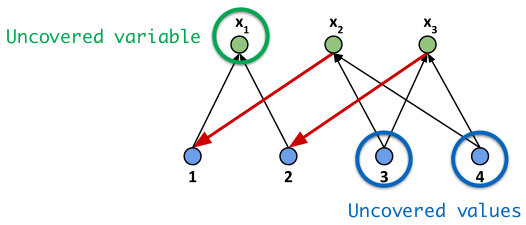
\includegraphics[width=8cm]{img/augmenting-paths.png}
            \caption{Augmenting paths}
        \end{figure}

    \item Stop when no more augmenting paths
\end{enumerate}

\paragraph{GAC}

\begin{description}
    \item \texttt{AllDifferent} is \textbf{GAC} iff all edge belong to
        a maximun matching covering all the variables
\end{description}

\begin{itemize}
    \item \textbf{Alternating path}

    \item \textbf{Alternating cycle}

\end{itemize}

\paragraph{Filtering}

\begin{enumerate}
    \item Find a maximun matching M
    \item if M.size != \#variables : \textcolor{red}{Fail}

    \item Find all edges belonging to an even \textbf{length alternating
        path} startint at a uncovered node (DFS or BDS)

        \paragraph{Alternating path}: start at an uncovered node and
        switch the edges in/out the matching. Change values
        of variables to stays maximum with different edges.

        \begin{figure}[!h]
            \centering
            %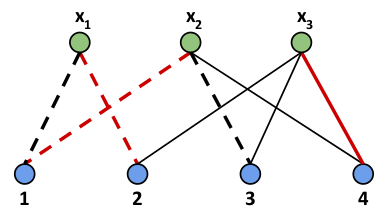
\includegraphics[width=8cm]{img/alternating.png}
            \caption{Alternating paths}
        \end{figure}

    \item Find all edges belonging to \textbf{alternating cycle} which
        correpons to the strongly connected components in the directed value
        graph

        \paragraph{Alternating cycle}: switch the edges in/out the matching.
        Exchange values of variables to stays maximum with different edges.

    \item Remove all edges/literals not in M and not found
\end{enumerate}

\paragraph{Incrementality of the filtering}
The value graph and maximum matching is keep in memory between calls to propagator.

\begin{tabular}{cm{12cm}}
When called
&
\begin{enumerate}
    \item Remove esdge not present anymore
    \item recompute maximum matching if necessary
    \item recompute GAC edges
\end{enumerate}
\end{tabular}

\subsubsection{Sum constraint}

\paragraph{NP-Hard}
Gac for a sum constraint is NP-Hard :

\paragraph{Proof} reduction of subset-sum to GAC for Sum
\begin{itemize}
    \item subset-sum: a NP-Hard problem for integer set ($S=\{a_1,\cdots, a_r\}$),
        does any non-empty subset of S sums to 0?

    \item reduction to GAC for Sum:
        \begin{lstlisting}[mathescape]
variables  $x_i$ with domains $\{0, a_i\}$
GAC on sum($[x_1,..., x_r], 0$)

if $D(x_i) = \{0\} \forall x_i$ : answer no
else: answer yes
\end{lstlisting}
\end{itemize}

\paragraph{Consequences} GAC propagator for sum is exponential (unless P=NP), so
the propagator is usually done with \textbf{Bound Consistency}

\paragraph{Bound consistency}

\begin{lstlisting}[mathescape]
propagate(){
    $\Delta = \emptyset$
    for( x $\leftarrow$ scope) {
        new_min = k - ($\sum_{(y \in scope, y \neq x)} y.max$)
        for( a $\leftarrow$ D(x) if a < new_min)
            $\Delta$ += (x, a)

        new_max = k - ($\sum_{(y \in scope, y \neq x)} y.min$)
        for( a $\leftarrow$ D(x) if a > new_max)
            $\Delta$ += (x, a)
    }
    return $\Delta$
}
\end{lstlisting}

\subsubsection{Element constraint}
%TODO

%TODO constraint slide 63 to 66



\subsection{Search}

CP mainly use DFS and at each
%TODO from slide 67 to the end











\subsection{Advantage}
\begin{itemize}
    \item Rich modeling language:
        \begin{itemize}
            \item  integer variables, set variables, graph variables
            \item  library of constraints (not necessarily linear)
        \end{itemize}
    \item  Fast prototyping
    \item  Easy to adapt/change a model
    \item  Extensible (you can create new constraints)
    \item  Great framework to hybridize with other techniques
\end{itemize}





\section{CP techniques}


\subsection{Scheduling CP}

\begin{center}
    \texttt{cumulative($[s_1,..., s_n], [d_1, ..., d_n], [e_1, ...,
    e_n], [c_1, ..., c_n], C$)}
\end{center}

\begin{itemize}
    \item $\forall_i: s_i + d_i = e_i$
    \item $\forall_t: \sum_{s_i \leq t < e_i} c_i \leq C$
\end{itemize}

\subsubsection{Sweep line algorithm}
It's use to compute the cumulated
profile and check that it does not exceed the capacity.


\begin{enumerate}
    \item \begin{tabular}{m{5cm}m{10cm}}
            \begin{itemize}
                \item One time point for start $(start, +capa)$
                \item One time point for end $(start, -capa)$ 
            \end{itemize}&
                    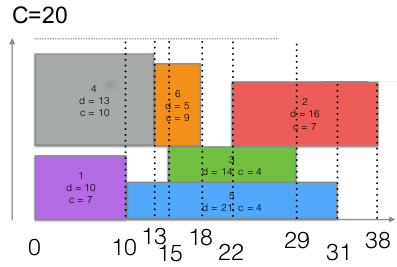
\includegraphics[width=7cm]{sweepLine}
                \end{tabular}


            \item \begin{tabular}{m{5cm}m{8cm}}
                    \begin{itemize}
                        \item Sort time points
                    \end{itemize}
                    &

                    (0,+7), (0,+10), (10,-7), (10,4), (13,-10), (13,9), (15,4), (18,-9), (22,7), (29,-4), (31,-4), (38,-7)
                \end{tabular}

            \item \begin{tabular}{m{5cm}m{10cm}}
                    \begin{itemize}
                        \item Sweep-line(t) = height of the profile at time $t$.
                    \end{itemize}
                    &
                    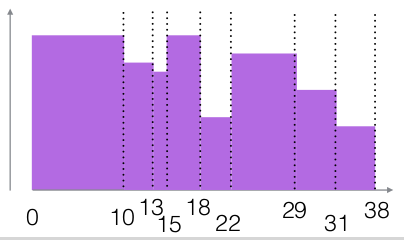
\includegraphics[width=7cm]{sweepLine2}
                \end{tabular}

                \begin{lstlisting}[mathescape]
input = eventQueue$[(time,c)]$
t = input.head.time   // Current time of the sweep line
h = 0                 //  current capacity of the sweep line 

while (input.nonEmpty) {
    while (input.nonEmpty && input.head.time == t){
    (time,c) = input.dequeue
    h = h + c
    }
    add (t,h) to the profile
    t = input.top.time
}
            \end{lstlisting}
    \end{enumerate}


\subsubsection{Optimistic Resource Profile}

\begin{tabular}{m{11cm}m{6cm}}
The optimistic resource profile is built based on the
\textbf{mandatory parts} which is the time where the activity will
use the resource whatever it final position.
&
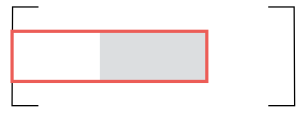
\includegraphics[width=4cm]{mandatory}
\end{tabular}

\begin{itemize}
    \item \textbf{Update minimum start time} at the earliest
        time such that it is not in conflict with the optimistic
        resource profile.

        \paragraph{Time complexity}: $O(n)$ per task since recource
        profile has $O(n)$ intervals. So, $O(n^2)$ overall.
\end{itemize}


\subsection{Large Neighborhood Search}

\begin{tabular}{m{12cm}m{3cm}}
    The diversification is the most weakness of CP for hard COPs.
    The idea of LNS is stuck for too long $\to$ jump in the search space
    by using restart!
    &
    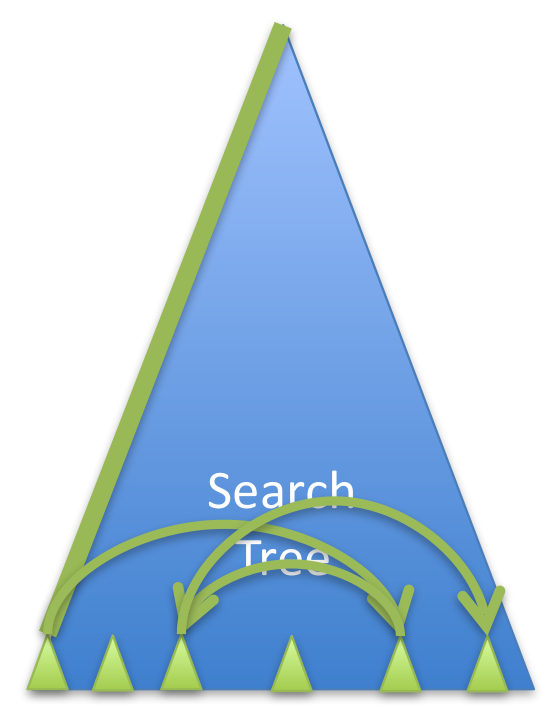
\includegraphics[width=2cm]{LNS}
\end{tabular}

\begin{tabular}{m{2cm}m{11cm}}
    Randomized restart & 
    \begin{itemize}
        \item Use some random decisions in your heuristic (value or variable)
        \item Use a limit on the search (number of backtracks or
            time)
        \item If no feasible solution is found within this limit,
            restart.
    \end{itemize}
\end{tabular}

\subsubsection{LNS work}

\begin{tabular}{m{10cm}m{6cm}}
    \begin{enumerate}

        \item Find a first initial solution, $S*$
        \item Randomly relax $S*$ and re-optimize with search limit

            Relax = fix some variables to their values in $S*$ and CP
            search the other

            \begin{itemize}
                \item A portion of the variables is selected (=\textbf{fragment})
                    and are relaxed to the \textbf{initial domain}
                \item The other variables are frozen to their value in the current solution
                \item A limited CP search \textbf{improving solutions}
            \end{itemize}

        \item Replace $S*$ by the best solution found
    \end{enumerate}

    &
    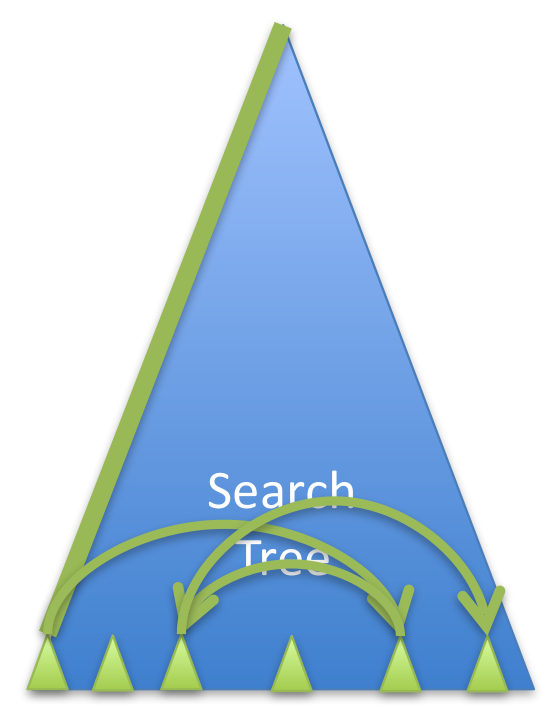
\includegraphics[width=6cm]{lns.png}
\end{tabular}

\paragraph{Advantages}
\begin{itemize}
    \item Good diversification if fragment well chosen $\Rightarrow$ no
        meta-heuristic needed (tabu,...) because neighborhood is large
        enough
    \item No need to design complex feasible neighborhoods because CP
        is in charge of feasibility

    \item Intensification with CP search and efficient 
        exploration of neighborhoods with CP
    \item Scalability of LS
\end{itemize}


\subsubsection{LNS parameters}
Parameters of LNS :
\begin{itemize}
    \item \textbf{Fragment size} and \textbf{time/backtrack limit}:
       strongly linked parameters because
       \begin{enumerate}
           \item fragment size determines neighborhood size
           \item limit determine the maximal effort to explore
       neighborhood.
       \end{enumerate}

       \paragraph{Note:} a good LNS should never be stopped only by the limit\ldots

       \paragraph{Adaptive versions}:
       \begin{enumerate}
           \item Fix a time/backtrack limit
           \item if neighborhood fully explored $\to$ increase fragment size
           \item else: decrease fragment size
       \end{enumerate}

    \item \textbf{fragment selection} (can be combined).

        Should contain important variables and related variables.

        \begin{itemize}
            \item \begin{tabular}{m{3cm}m{10cm}}
                    Random selection &
                \begin{itemize}
                    \item Surprisingly good
                    \item Generic
                    \item Excellent diversification
                    \item Intensification from CP search
                \end{itemize}
            \end{tabular}

        \item \begin{tabular}{m{3cm}m{10cm}}
                    Specific selection &
                \begin{itemize}
                    \item Only for one problem
                    \item Use knowkedge of the problem to select variables
                    \item Usually randomized to some extend
                \end{itemize}
            \end{tabular}
        \end{itemize}
\end{itemize}

\subsubsection{QAQ}
%TODO LNS relax

\subsubsection{Vehicle routing}
%TODO explain

\subsubsection{Cutting stock}
%TODO column generation











\section{Derivative free optimization}
Usually when we try to optimize a function with a continuous domain we use derivative.
However it is not always possible because:\newline
1) The gradient is not computable\newline
2) We dont know the objective function\newline
3) The gradient is to expensive to compute\newline
4) We don't know how to compute the gradient\newline

We can use Derivative free optimization.
We dont know the objective function but we have comparison function that allows us to compare solutions.

\subsection{Grid Search}
Since the domain is continuious we can't compare every point. To solve this problem we will cut each dimension of the domain in m. We evaluate eaach one of these combination and we output the minimum.
We will always have $m^n$ evaluation(because we have n dimensions that we cut in m parts).
We could do a smarter grid search but iteratively perform a grid search and then reduce our domaine for the minimum output area we have found.
So if we do i iterations we will have $i * m^n$ evaluations od the objective.
\subsection{Directional Direct Search}
Global idea\newline
Test a sample of points in specified directions around the iterate.
If a point is better, select it as next iterate.\newline
This algorithm consiste of two steps:\newline
1)Poll step:\newline
We test the different possibilities and go to a better one(with our comparaison function)\newline
2)Mesh parameter update:\newline
We update the size of the step we want to perform.\newline
\subsubsection{Poll step}
We define a set D of positive bases that is going to define the direction we will explore.
Exemple:\newline
For a 3D space D is :\newline
$e_1$ = (1,0,0)\newline
$e_2$ = (0,1,0)\newline
$e_3$ = (0,0,1)\newline

How to build a new point:\newline
$x_(new) = x+\alpha*d (with d in D)$
\subsubsection{Mesh Parameter Update}
Two cases:\newline
1)Iteration declared sucessfull(we found a better solution with the comparaison function)\newline
2)





\section{Bi-objective}
%TODO slides 11




\end{document}
